\documentclass[11pt,a4paper]{article}

% ===== Encoding and fonts =====
\usepackage[utf8]{inputenc}
\usepackage[T1]{fontenc}

% ===== Page geometry =====
\usepackage[top=88.9pt, bottom=36.0pt, left=56.7pt, right=39.5pt]{geometry}

% ===== Packages =====
\usepackage{amsfonts}
\usepackage{amsmath}
\usepackage{amssymb}
\usepackage{float}
\usepackage{graphicx}
\usepackage[colorlinks=true,linkcolor=blue,urlcolor=blue]{hyperref}
\usepackage[dvipsnames,svgnames,x11names]{xcolor}

% ===== Spacing =====
\usepackage{setspace}
\setlength{\parindent}{0pt}
\setlength{\parskip}{6pt}

% ===== Custom colors =====
\author{Dr Santosh Kumar Das}

\begin{document}

\begin{figure}[H]
\centering

\includegraphics[width=0.65\linewidth]{images/image_p1_1.jpeg}
\end{figure}

\section*{The Department of Computer Science \& Engineering }

{\LARGE (CSE) 
(Even Sem 2024-25) }

{\LARGE Project/ Internship Report On }

\begin{center}
{\LARGE \textbf{“Credit Card Fraud Detection using Machine }}
\end{center}

\begin{center}
{\LARGE \textbf{Learning”” }}
\end{center}

\subsection*{(Project Stage-I (Mini Project/ Industrial Training), CSE-601-P1) }

\subsection*{Submitted to }

\subsection*{The Department of CSE }

{\large In partial fulfillment of the requirements for the award of the BTech CSE by }

{\small Abhishek Chatterjee (SBU221026), Sem-6th, Section-A }

\begin{center}
{\large Shivani Deonath (SBU221482), Sem-6th, Section-D 
Jiten kr Sarkhel (SBU220845), Sem-6th, Section-A }
\end{center}

\begin{center}
{\large Under the guidance of }
\end{center}

\begin{center}
{\large Dr. Dipti Kumari 
Associate Professor 
Department of CSE }
\end{center}

{\Large Sarala Birla University, Ranchi }

\begin{center}
{\LARGE \textbf{May, 2025 }}
\end{center}

\newpage

{\Large Certificate }

Certified that Abhishek Chatterjee (SBU221026), Shivani Deonath (SBU221482) and Jiten kr 

Sarkhel (SBU220845) of BTech CSE (AI\&ML, DS\&CC) 6th 2022-26, have carried out the 

research work presented in this project entitled “Credit Card Fraud Detection using Machine 

\subsubsection*{Learning” for the award of (BTech-CSE/AI/ BCA/ MCA/ MTech-CSE degree) / (Diploma-}

CSE) from Sarala Birla University, Ranchi under my supervision during Even Sem 2024-25 session. 

The project embodies result of original work and studies carried out by Student himself and the contents of 

{\small the project do not form the basis for the award of any other degree to the candidate or to anybody else. }

{\Large Sign: \_\_\_\_\_\_\_\_\_\_ }

\[
  Sign: __________
\]

Date: 

\subsubsection*{(Dr. Dipti Kumari) }

Associate Professor, 

Department of CSE 

\begin{flushright}
Sarala Birla University, Ranchi 
\end{flushright}

Page | 1  

\newpage

\section*{Declaration }

We, Abhishek Chatterjee(SBU221026), Shivani Deonath(SBU221482) and Jiten kr 

\subsubsection*{Sarkhel(SBU220845), student of BTech CSE (AI\&ML, DS\&CC)-6th, Batch(2022-26), hereby }

declare that the report titled “ Credit Card Fraud Detection using Machine Learning” which is 

submitted by us to the department of CSE , Sarala Birla University Jharkhand, in partial fulfillment 

of the requirement for the award of degree/ diploma in “BTech CSE(AI\&ML, DS\&CC)-” , has not 

been previously formed the basis for the award of any degree, diploma or other similar title or 

recognition. We further declare that the report is written by us and no part of the report is copied from 

any source(s) without being duly acknowledged.  

Signature: 
Signature: 
Signature: 
Date:                                                   Date:                                        Date: 

\subsubsection*{Abhishek Chatterjee  
            Shivani Deonath 
           Jiten kr Sarkhel }

\subsubsection*{SBU221026 
SBU221482 
SBU220845 }

Page | 2  

\newpage

{\Large Acknowledgement }

I express my sincere gratitude to my project guide Dr. Dipti Kumari for her able guidance, 
continuous support and cooperation throughout my project, without which the present work would 
not have been possible. My endeavor stands incomplete without dedicating my gratitude to him/ she; 
he / she has contributed a lot towards successful completion of my project work. 

I would like to acknowledge my indebtedness and deep sense of gratitude to Dr. Pankaj Kr Goswami 
sir, Dean-FoECS, SBU, Dr. Biswarup Samanta sir, Asso. Dean-FoECS \& HoD – CSE\&CA, SBU 
and my Program Coordinator, Dr. Dipti Kumari madam, to encourage me to the highest peak and 
to provide me the opportunity to prepare the project. 

I would also like to express my sincere thanks towards my teachers at SBU and my family and friends 
for their unending support, and tireless effort that kept me motivated throughout the completion of 
this project. 

Name of the Student:  Abhishek Chatterjee, Shivani Deonath, Jiten kr Sarkhel 

Enrollment Number:  SBU221026, SBU221482, SBU220845 

Program:  BTech CSE (AI\&ML, DS\&CC) 

Semester:  6th 

Section:  A \& D 

Batch:  2022-26 

Page | 3  

\newpage

\section*{Table of Contents }

{\large Topic  
          Page Number 
• Title Page ……………………………………………………………………...     
• Certificate ……………………………………………………………………..    1 
• Declaration ……………………………………………………………………    2 
• Acknowledgement ……………………………………………………………    3 
• Table of Contents ……………………………………………………………..    4 
• Project Synopsis ………………………………………………………………   5  
• List of Figures…………………………………………………………………    6 
1. 
INTRDOUCTION…………………………………………………………   07 - 11 
• 
Theoretical Background  
• 
Objective of the Project  
• 
Scope of the study 
• 
Limitations of the Study 
2. 
PROBLEM ANALYSIS ………………………………………………….   12 - 34 
• 
PROBLEM DEFINATION 
• 
REQUIREMENT ANALYSIS AND DEVELOPMENT }

a. Functional Requirement 
b. Nonfunctional Requirement 
c. Goals of Implementation 
• 
DATA ANALYSIS AND DATA VISUALISATION 
3. 
SYSTEM IMPLIMENTATION DETAILS ………………………………  35 - 36 
• 
Methodology Adopted 
• 
Hardware and Software Used 
4. 
DESIGN           ……………………………………………………………  37 - 40 
• 
Flowchart 
• 
Entity Relationship Diagram 
5. 
IMPLEMENTATION …………………………………………….. …….   41 - 44 
6. 
RESULT………………………………………………………………….    45 - 50 
• 
Experimental Result 1 (Output Screenshot) 
• 
Experimental Result 2 (Output Screenshot) 
• 
Experimental Result n (Output Screenshot) 
7. 
CONCLUSION ……………………………………….………………..      51  
8.      FUTURE SCOPE ………………………………………………………      52 - 54 
  9.      LIMITATIONS ………………………………………………………….     55 - 57 
 10.     ANNEXURE – I:  …………………………………………………………   58      
                References  
 11.     ANNEXURE – II:  …………………………………………………………  59      
                Weekly Progress Reports (All original copies of WPRs)  

Page | 4  

\newpage

\begin{figure}[H]
\centering

\includegraphics[width=1.00\linewidth]{images/image_p6_2.jpeg}
\end{figure}

\section*{THE DEPARTMENT OF CSE }

\subsection*{       PROJECT SYNOPSIS }

\textbf{Student Name: Abhishek Chatterjee, Shivani Deonath, Jiten kr Sarkhel  
Enrollment No.: SBU221026, SBU221482, SBU220845 
Program \& Branch: BTech CSE (AI\&ML, DS\&CC) 
Batch: 2022-2026, Semester: 6th, Section:  A, D 
Academic Session: Even Semester 2024-25 
Project Guide Details: }

• Guide Name: Dr. Dipti Kumari 
• Designation: Associate Professor, CSE, SBU 

\subsubsection*{Project Information }

\textbf{1. Course Title: Project Stage-I (Mini Project/ Industrial Training) 
2. Courses Code: CSE-601-P1                                              
3. Credit Unit: 2 
4. Project/ Internship Duration:  }

\textbf{• 
Date of Project Commencement: 21st March, 2024 
• 
Date of Project Completion: 21st April, 2025 
5. Approved Project Title (to be duly approved by the Project Guide): 
“Credit Card Fraud Detection using Machine Learning” 
6. Objectives:  
Develop a machine learning model for real-time credit card fraud detection using classification and anomaly 
detection techniques, handling class imbalance with SMOTE. Evaluate performance using metrics like ROC-
AUC and F1-score, and deploy with a user-friendly interface for practical financial security applications. 
7. Methodology to be adopted: }

• 
Data Collection \& Preprocessing: Used Kaggle data, cleaned, scaled, applied SMOTE. 
• 
Model Building \& Evaluation: Trained Random Forest, evaluated with key metrics. 
• 
Deployment \& Documentation: Built Streamlit web app, documented project. 
8. Brief Summary of the project: 
This project detects credit card fraud using anonymized, imbalanced data by applying preprocessing, 
SMOTE oversampling, and a Random Forest model. It is evaluated with key metrics and deployed through 
an easy-to-use interface to help reduce fraud. 
Signature with date 
   Signature of Industry Guide, if any  
     Signature with date 
   (Student) 
          (Project Guide) 

Page | 5  

\newpage

\begin{center}
{\Large List of Figures }
\end{center}

1. Class Distribution code. 

2. Class Distribution plot. 

3. Class Distribution data. 

4. Amount Distribution by class code. 

5. Amount Distribution by class plot. 

6. Correlation matrix code. 

7. Correlation matrix plot. 

8. Time vs Amount plot code. 

9. Time vs Amount plot plot. 

10. Count plot for class code. 

11. Count plot for class plot. 

12. Transaction amount distribution code. 

13. Transaction amount distribution plot. 

14. Boxplot of Amount by class code. 

15. Boxplot of Amount by class plot. 

 16. Time distribution of transactions code. 

 17. Time distribution of transactions plot. 

18. Time vs Amount scatter, colored by class code. 

19. Time vs Amount scatter, colored by class plot. 

20. Distribution of top correlated features code. 

21. Distribution of top correlated features 1 plot. 

22. Distribution of top correlated features 2 plot. 

23. Distribution of top correlated features 3 plot. 

24. Distribution of top correlated features 4 plot. 

25. plot the pie chart 1 code. 

26. plot the pie chart 1 plot. 

27. plot the pie chart 2 code. 

28. plot the pie chart 2 plot. 

29. plot the pie chart 3 code. 

30. plot the pie chart 3 plot. 

31. plot the pie chart 4 code. 

32. plot the pie chart 4 plot. 

33. Fraud Distribution by Hour code. 

34. Fraud Distribution by Hour plot. 

Page | 6  

\newpage

\section*{1. INTRODUCTION }

\subsection*{1.1 THEORETICAL BACKGROUND }

         Credit card fraud is one of the most pervasive threats in the digital payment ecosystem 

today, contributing to substantial financial losses for consumers, merchants, and financial 
institutions worldwide. As e-commerce and online financial transactions grow rapidly, 
fraudsters continually evolve their methods to exploit vulnerabilities in payment systems. 
Consequently, detecting fraudulent transactions with speed and accuracy has become a 
critical objective for organizations handling sensitive financial data. 

         Traditionally, fraud detection systems relied on manually defined rules and heuristic-based 

approaches. These systems, while effective to an extent, lack the adaptability and 
sophistication required to counter modern fraud tactics. They often result in either a high 
number of false positives—flagging legitimate transactions as fraud—or a failure to detect 
subtle and emerging fraudulent behavior. As such, the industry has pivoted towards data-
driven and intelligent systems, particularly machine learning, to tackle this issue. 

         Machine learning (ML) offers a dynamic approach to fraud detection by analyzing patterns, 

behaviors, and anomalies in transactional data. In this project, a supervised learning 
approach is adopted using the Random Forest classifier, which is known for its robustness 
and performance in classification tasks. The dataset used originates from Kaggle and 
includes 284,807 credit card transactions, of which only 492 are classified as fraudulent. 
This severe class imbalance presents unique challenges in training predictive models. 

         To address this imbalance, the Synthetic Minority Over-sampling Technique (SMOTE) is 

applied. SMOTE generates synthetic examples of the minority class (fraud) to balance the 
dataset and reduce model bias. Before applying SMOTE, features like 'Time' and 'Amount' 
are scaled using StandardScaler to ensure uniformity across data distributions. Additionally, 
the features V1 to V28—extracted using Principal Component Analysis (PCA)—represent 
the anonymized transaction attributes and form the core predictors for the model. 

         The project workflow encompasses data preprocessing, model training, performance 

evaluation, and deployment. The trained model is evaluated using appropriate metrics such 
as precision, recall, F1-score, and ROC-AUC, which are better suited to imbalanced 
classification scenarios. The deployment phase utilizes Streamlit to build a web-based 
interface where users can input transaction attributes and receive instant fraud detection 
feedback. 

         Furthermore, the application is designed to provide not only binary predictions (fraudulent 

or legitimate) but also confidence scores to support decision-making. The modular structure 
of the codebase ensures scalability, maintainability, and ease of integration into larger fraud 
detection systems. 

        This theoretical framework highlights the role of supervised learning in the financial security 

{\small domain and emphasizes the importance of preprocessing techniques, evaluation metrics, and 
real-time usability in deploying fraud detection systems. As cyber threats continue to evolve, 
the combination of advanced machine learning algorithms and real-time data analysis 
remains a powerful defense mechanism against credit card fraud. }

Page | 7  

\newpage

1.2 OBJECTIVE OF THE PROJECT 
The objective of this project is to design and develop a robust, intelligent system that can 
automatically detect fraudulent credit card transactions using machine learning. With the 
increasing reliance on digital transactions, the need for efficient, scalable, and accurate fraud 
detection mechanisms has never been greater. This project is aimed at addressing that need 
through the development of a practical and technically sound solution. 
One of the key challenges in credit card fraud detection is the imbalance in data—fraudulent 
transactions represent a very small fraction of the total. This makes traditional classifiers 
biased toward predicting the majority class (non-fraudulent transactions), often missing the 
crucial minority class. Thus, one of the primary objectives of this study is to mitigate this 
imbalance using techniques like SMOTE (Synthetic Minority Over-sampling Technique) 
that allow the model to learn from underrepresented fraudulent cases. 
Another important goal is to build a machine learning pipeline that is not only accurate but 
also interpretable and maintainable. For this, we use Random Forest Classifier, which offers 
a balance between predictive performance and model transparency. The model's output is 
evaluated using classification metrics tailored to imbalanced datasets, including precision, 
recall, F1-score, and ROC-AUC. These metrics help in understanding the trade-offs between 
catching frauds and avoiding false alarms. 
The project also places significant emphasis on usability and accessibility. The trained 
model is deployed using a lightweight web framework, Streamlit, which allows real-time 
fraud prediction through a user-friendly interface. This interface accepts specific transaction 
inputs (features) and returns a prediction along with the probability of fraud. Such an 
approach not only makes the system accessible to non-technical users but also showcases 
how machine learning can be integrated into live financial systems. 
Furthermore, the objective extends to educational and research purposes. The entire 
development process—from data preprocessing, model training, evaluation, and 
deployment—serves as a comprehensive case study on solving real-world classification 
problems with skewed data. This can benefit students, researchers, and practitioners in the 
domain of artificial intelligence, data science, and cybersecurity. 
The project also aims to demonstrate modularity and scalability. By structuring the project 
into separate components (data loading, preprocessing, training, prediction, UI), it becomes 
easier to scale or update individual parts without rewriting the entire system. For example, a 
different model can be swapped in later stages for performance comparison, or the dataset 
can be extended with new fraud types for retraining. 
In summary, the objectives of this project can be broadly categorized as follows: 
• 
Technical Objective: To build a high-performing, real-time fraud detection system 
using machine learning. 
• 
Practical Objective: To develop a deployable interface that helps identify fraudulent 
transactions effectively. 
• 
Analytical Objective: To use meaningful performance metrics for evaluating fraud 

Page | 8  

\newpage

detection accuracy. 
• 
Educational Objective: To serve as a learning resource for end-to-end ML pipeline 
development. 
• 
Scalability Objective: To ensure modular code that can be reused and extended in real-
world applications. 
Achieving these objectives not only contributes to mitigating the impact of credit card fraud 
but also provides a reusable framework for similar classification problems in other domains 
such as insurance fraud, loan defaults, and cyber threat detection 

\subsection*{  1.3 SCOPE OF THE STUDY }

The scope of this project extends across multiple phases of the machine learning lifecycle, including 
data acquisition, preprocessing, model training, performance evaluation, and real-time deployment. 
The study aims to address both the technical and practical aspects of credit card fraud detection by 
implementing a robust and modular machine learning system. 

This project utilizes a publicly available, real-world credit card transaction dataset that includes 
anonymized features derived using Principal Component Analysis (PCA). The dataset offers a 
realistic setting with severe class imbalance, as fraudulent transactions account for only a tiny fraction 
of the total. This makes it a suitable testbed for evaluating machine learning algorithms under 
challenging conditions. 

The implementation focuses on the supervised classification paradigm using the Random Forest 
algorithm, chosen for its interpretability, performance, and resistance to overfitting. The model is 
trained on preprocessed data, where features such as 'Time' and 'Amount' are standardized and class 
imbalance is mitigated using the Synthetic Minority Over-sampling Technique (SMOTE). These 
preprocessing steps are crucial for ensuring the model learns meaningful patterns from the minority 
class. 

The system is also designed to be interactive and accessible. A lightweight user interface is developed 
using Streamlit, allowing real-time fraud detection based on user-input transaction features. This UI 
not only demonstrates the practical applicability of the model but also provides a foundation for future 
integration with real-world payment systems. 

The scope further includes evaluating the model using a comprehensive set of metrics. Metrics such 
as precision, recall, F1-score, and ROC-AUC are used to assess the model's performance, particularly 
its ability to detect frauds without producing excessive false positives. Visualizations like confusion 
matrices and ROC curves help interpret and validate the results. 

Additionally, the project emphasizes modular development, enabling scalability and maintainability. 
Each component of the project—data preprocessing, model training, evaluation, and prediction—is 
encapsulated in separate scripts, allowing independent updates or enhancements. This makes the 
system adaptable for future extensions such as introducing new algorithms, real-time data ingestion, 
or advanced visualization dashboards. 

Page | 9  

\newpage

The educational aspect of the project is also noteworthy. The step-by-step implementation, combined 
with clean code organization and documentation, makes the system an excellent reference for students 
and researchers working on similar classification problems or fraud detection systems. 

In summary, the scope of this study includes: 

• 
Utilizing a real-world anonymized dataset for building and validating a fraud detection model. 

• 
Implementing preprocessing techniques like scaling and SMOTE to prepare data for machine 
learning. 

• 
Training a Random Forest classifier and evaluating its effectiveness using domain-relevant 
metrics. 

• 
Developing a user-friendly web application for real-time fraud prediction. 

• 
Demonstrating a modular and scalable design suitable for future enhancements and 
production-level deployment. 

• 
Providing educational value through a clearly documented and replicable machine learning 
pipeline. 

The project thus lays a robust foundation for more advanced and integrated fraud detection systems 
capable of learning from evolving threats in real-time financial environments. 

for more advanced fraud detection systems that could incorporate continuous learning, unsupervised 
anomaly detection, and integration with live banking APIs. 

\subsection*{1.4 LIMITATIONS OF THE STUDY }

While this project has successfully implemented a practical and technically robust fraud detection 
system, it is essential to acknowledge certain limitations that may impact its real-world applicability 
and performance. 

Firstly, the dataset used for training and evaluation is anonymized and sourced from a specific 
financial institution over a short period. As a result, it may not fully represent the diverse and 
dynamic nature of credit card transactions across different banks, countries, and transaction 
platforms. This constraint limits the generalizability of the model when applied to real-world, 
heterogeneous financial environments. 

Secondly, the model has been trained on historical data and lacks adaptive capabilities. Fraud 
patterns evolve rapidly, and a static model may become outdated over time. Although retraining the 
model periodically can help, it is not a substitute for real-time learning. Incorporating continuous or 
online learning methods could improve the system's ability to respond to emerging fraud tactics. 

Another limitation lies in the deployment layer. While Streamlit provides an accessible and 
interactive interface for demonstration, it is not designed for high-throughput or production-grade 
applications. In real-world use cases, fraud detection systems need to process large volumes of data 
with minimal latency, often integrating with payment gateways or banking systems. Thus, a more 

Page | 10  

\newpage

scalable deployment framework such as Flask, FastAPI, or cloud-native services would be required 
for commercial deployment. 

Moreover, the project solely employs supervised learning techniques. While these methods are 
effective when labeled data is abundant, they are limited in uncovering unknown fraud patterns or 
zero-day anomalies. The absence of unsupervised or semi-supervised learning techniques means the 
model is less capable of identifying new or evolving forms of fraud that are not represented in the 
training data. 

In terms of model evaluation, although metrics like ROC-AUC and F1-score are insightful, they 
may not fully capture the cost implications of false positives and false negatives in fraud detection. 
In financial domains, a false negative (i.e., a missed fraud) can lead to substantial monetary losses, 
while a false positive may inconvenience a genuine customer. Therefore, future iterations of the 
model could include cost-sensitive learning strategies to address this issue more effectively. 

Lastly, ethical considerations related to data usage and privacy are beyond the scope of this project. 
Fraud detection systems deal with sensitive user data, and their deployment must comply with data 
protection regulations like GDPR. While this project handles anonymized data, deploying a real-
time system would necessitate strict adherence to ethical and legal standards. 

In conclusion, while the project provides a strong foundation for credit card fraud detection using 
machine learning, addressing these limitations is crucial for transitioning from a prototype to a real-
world, production-grade solution. Future work can involve adapting the system to real-time streams, 
incorporating anomaly detection, improving scalability, and aligning with ethical standards. 

Page | 11  

\newpage

\section*{2. PROBLEM ANALYSIS }

\subsection*{    2.1 PROBLEM DEFINATION  }

\subsection*{2.1.1 Introduction }

In the contemporary digital economy, credit card transactions form a fundamental component of financial 
operations across the globe. The convenience and efficiency of credit card use have led to their widespread 
adoption in both physical and online purchases. However, this widespread adoption has also opened the door 
for a growing number of fraudulent activities, posing a significant threat to consumers, merchants, and 
financial institutions alike. As transactions increasingly shift to digital platforms, the magnitude and 
sophistication of credit card fraud continue to escalate, necessitating the development of automated, accurate, 
and real-time fraud detection systems. 

The primary objective of a credit card fraud detection system is to accurately identify and prevent 
unauthorized or illegitimate transactions before they cause financial damage. This involves analyzing large 
volumes of transactional data to uncover subtle patterns that may signify fraud. Given the speed at which 
transactions occur, especially in online environments, fraud detection must be executed in real-time and with 
minimal false positives to avoid disrupting genuine user experiences. 

This project aims to address these challenges by developing an intelligent fraud detection system based on 
supervised machine learning. Specifically, it focuses on classifying transactions as either legitimate or 
fraudulent based on historical data, using classification algorithms capable of handling highly imbalanced 
datasets and deploying the model through a real-time, user-friendly interface. 

\subsubsection*{2.1.2 Nature of the Problem }

Credit card fraud detection is fundamentally a binary classification problem where each transaction must be 
labeled as either fraudulent or legitimate. The complexity of this task arises due to the following key 
challenges: 

\subsubsection*{a) Imbalanced Data }

In typical transaction datasets, fraudulent transactions represent less than 1\% of the data. This extreme class 
imbalance causes conventional machine learning algorithms to become biased toward the majority class 
(non-fraudulent), which may lead to a high overall accuracy but poor performance in detecting actual frauds. 
Misclassifying a fraudulent transaction as legitimate (false negative) can have far more serious consequences 
than the inverse. 

\subsubsection*{b) Evolving Fraud Patterns }

Fraudsters continuously adapt their strategies to bypass detection systems. Traditional rule-based systems 
become obsolete quickly as they are unable to detect new or evolving fraud tactics. An effective fraud 
detection system must be able to learn from data and generalize to previously unseen patterns. 

\subsubsection*{c) Real-Time Detection Requirements }

Given the rapid pace of online and digital transactions, a delay in fraud detection can result in irreversible 
financial loss. Hence, the system must not only be accurate but also fast enough to operate in real-time or 
near-real-time environments. 

\subsubsection*{d) High Cost of Errors }

Page | 12  

\newpage

The consequences of false negatives (frauds missed by the system) can result in substantial monetary losses. 
On the other hand, false positives (legitimate transactions flagged as fraud) can frustrate customers and lead 
to reputational damage. The system must balance sensitivity and specificity to minimize both types of errors. 

\subsubsection*{e) Privacy and Security }

Fraud detection systems must be designed to handle sensitive financial data responsibly, ensuring that data 
privacy laws and ethical standards are upheld throughout the process. 

\subsubsection*{2.1.3 Problem Statement }

The core problem addressed in this project can be articulated as follows: 

\textbf{"To design and implement a machine learning-based credit card fraud detection system capable of 
accurately identifying fraudulent transactions in real-time, despite challenges such as data imbalance, 
evolving fraud patterns, and the need for high-speed processing." }

This problem encompasses data acquisition, preprocessing, model training, performance evaluation, and 
deployment—all while ensuring usability and scalability for practical use. 

\subsubsection*{2.1.4 Proposed Solution Overview }

To address the defined problem, the project proposes a machine learning-driven approach with the following 
key components: 

1. Data Acquisition: Use a publicly available credit card transaction dataset (e.g., from Kaggle), which 

contains anonymized features derived from PCA, along with transaction amount, time, and class 
labels. 

2. Preprocessing: 

\begin{center}
o 
Scale continuous variables like Time and Amount using StandardScaler. 
\end{center}

o 
Address class imbalance using SMOTE (Synthetic Minority Over-sampling Technique). 

3. Model Selection and Training: 

o 
Use the Random Forest Classifier, known for its robustness and interpretability. 

o 
Train the model using stratified sampling and cross-validation to ensure balanced learning. 

4. Evaluation: 

o 
Evaluate the model using performance metrics such as Precision, Recall, F1-score, and 
ROC-AUC, which are more informative in imbalanced datasets. 

5. Deployment: 

o 
Deploy the model using Streamlit to provide a web-based interface for real-time fraud 
predictions. 

o 
The interface will allow users to input transaction details and receive a prediction label 
(fraud/legit) along with a probability/confidence score. 

Page | 13  

\newpage

6. Documentation and Scalability: 

o 
Ensure that the system is well-documented, modular, and easily extensible for future 
enhancements, such as using ensemble models or integrating with live banking APIs. 

\subsubsection*{2.1.5 Benefits of the Proposed System }

• 
Improved Fraud Detection Accuracy: Leveraging machine learning to detect patterns that are not 
easily observable with rule-based systems. 

• 
Real-Time Capability: Predictions are generated within seconds of receiving inputs. 

• 
User-Friendly Interface: A lightweight web application makes the system usable even by non-
technical personnel. 

• 
Educational Value: The system serves as a complete case study for data preprocessing, modeling, 
evaluation, and deployment in machine learning. 

• 
Scalable and Modular Design: Components are separated logically, allowing integration with 
larger financial systems or APIs in future. 

\subsubsection*{2.1.6 Relevance to Industry and Academia }

This project is highly relevant to both academia and industry. In academic research, it contributes to the field 
of machine learning for imbalanced classification and fraud analytics. In industry, it provides a prototype 
framework that could be adapted for use by financial institutions to enhance fraud detection systems. 

Moreover, the system demonstrates practical challenges and solutions encountered in building real-world AI 
applications, including ethical considerations, interpretability, and integration barriers—topics of increasing 
importance in modern computer science education. 

\subsection*{2.2 REQUIREMENT ANALYSIS AND DEVELOPMENT }

This section outlines the software requirements critical for the successful implementation of the Credit Card 
Fraud Detection System. The requirements are divided into two categories—Functional and Non-
Functional—and are followed by the Goals of Implementation, each expanded to provide a comprehensive 
understanding of the system expectations. 

\subsubsection*{2.2.1 Functional Requirements }

Functional requirements define the specific behavior and functions the system must perform to fulfill its 
objectives. For this project, the functional requirements focus on the core capabilities of the fraud detection 
system, from data processing and model training to prediction and UI interaction. 

Page | 14  

\newpage

\subsubsection*{2.2.1.1 Data Loading and Preprocessing }

• 
The system shall load transaction data from a .csv file. 

• 
The system shall normalize continuous variables (e.g., Time and Amount). 

• 
The system shall handle missing values (if any) appropriately. 

• 
The system shall apply SMOTE to balance the class distribution. 

\subsubsection*{2.2.1.2 Model Training }

• 
The system shall allow training of a machine learning model (Random Forest). 

• 
The system shall split the data into training and testing subsets. 

• 
The system shall store the trained model using joblib for reuse. 

\subsubsection*{2.2.1.3 Evaluation }

• 
The system shall generate performance metrics: Accuracy, Precision, Recall, F1-Score, and ROC-
AUC. 

• 
The system shall display a confusion matrix and ROC curve. 

• 
The system shall log evaluation results for further review. 

\subsubsection*{2.2.1.4 Prediction Module }

• 
The system shall accept a set of features (V1-V28, Time, Amount) as input. 

• 
The system shall use the trained model to return a binary classification: 0 (Legit) or 1 (Fraud). 

• 
The system shall return the probability (confidence score) associated with each prediction. 

\subsubsection*{2.2.1.5 User Interface (UI) }

• 
The system shall provide a web interface via Streamlit. 

• 
The UI shall allow users to enter transaction inputs manually. 

• 
The UI shall return fraud predictions and highlight results. 

• 
The UI shall be accessible via a web browser. 

\subsubsection*{2.2.1.6 Reporting and Logging }

• 
The system shall log input transactions and corresponding predictions. 

• 
The system shall allow exporting evaluation metrics as a report. 

• 
The system shall notify the user of any abnormal input. 

\subsubsection*{2.2.1.7 Modularity and Extensibility }

• 
Each module (preprocessing, training, evaluation, prediction) shall be developed independently. 

• 
The system shall support replacing the machine learning model with another classifier (e.g., Logistic 
Regression). 

Page | 15  

\newpage

• 
The codebase shall follow clean coding practices and be version-controlled. 

\subsubsection*{2.2.2 Non-Functional Requirements }

Non-functional requirements define the performance attributes and constraints of the system. These 
requirements address how the system operates, ensuring usability, security, maintainability, and scalability. 

\subsubsection*{2.2.2.1 Performance }

• 
The system shall make predictions in under 2 seconds for individual inputs. 

• 
The model training process shall be optimized to complete within 5 minutes on a standard CPU. 

\subsubsection*{2.2.2.2 Usability }

• 
The system shall be user-friendly for non-technical users. 

• 
The UI shall display error messages and guidance where needed. 

• 
The layout shall be minimalistic with labeled inputs and readable output. 

\subsubsection*{2.2.2.3 Reliability }

• 
The system shall produce consistent results on repeated runs of the same input. 

• 
The model shall be evaluated with cross-validation to ensure generalizability. 

\subsubsection*{2.2.2.4 Scalability }

• 
The code structure shall allow future upgrades with additional features or new datasets. 

• 
The backend logic shall be modular enough to plug in alternative classifiers or ensemble methods. 

\subsubsection*{2.2.2.5 Maintainability }

• 
The system shall use proper documentation and in-line comments. 

• 
Each script/module shall be stored in a dedicated folder with a clear naming convention. 

• 
A README file shall be available for developer onboarding. 

\subsubsection*{2.2.2.6 Portability }

• 
The system shall be executable on Windows and Linux platforms. 

• 
Dependencies shall be listed in a requirements.txt file. 

• 
A setup script or environment installation guide shall be included. 

\subsubsection*{2.2.2.7 Security }

• 
Input data shall be validated to prevent injection or malformed entries. 

• 
Prediction logs shall not store personally identifiable information (PII). 

• 
Model and data files shall be stored in restricted-access folders. 

\subsubsection*{2.2.2.8 Availability }

Page | 16  

\newpage

• 
The system shall be available for demonstration and local usage 24/7 (non-cloud). 

• 
System downtime during training or batch updates shall be minimized. 

\subsubsection*{2.2.3 Goals of Implementation }

This section outlines the overarching goals that guide the implementation process, ensuring alignment 
between project deliverables and stakeholder expectations. 

\subsubsection*{2.2.3.1 Technical Goals }

• 
Develop a robust, accurate, and reproducible fraud detection pipeline. 

• 
Utilize machine learning techniques suited for imbalanced classification problems. 

• 
Ensure the system handles real-world constraints such as speed, scale, and interpretability. 

\subsubsection*{2.2.3.2 Usability Goals }

• 
Provide a user interface that is intuitive and responsive. 

• 
Minimize the need for technical intervention during prediction. 

• 
Present outputs in a manner that is clear and actionable for decision-makers 

\subsubsection*{2.2.3.3 Deployment Goals }

• 
Enable seamless model deployment through Streamlit. 

• 
Support easy migration to cloud platforms for future scalability. 

• 
Allow integration with external systems via API in extended versions. 

\subsubsection*{2.2.3.4 Educational Goals }

• 
Create a full-stack reference project for students and researchers. 

• 
Demonstrate best practices in machine learning pipeline construction. 

• 
Enable experimentation and learning through clear modularization. 

\subsubsection*{2.2.3.5 Innovation Goals }

• 
Promote the use of machine learning for financial fraud risk management. 

• 
Showcase the importance of real-time prediction and explainable AI in fintech. 

• 
Inspire future enhancements including dynamic learning and unsupervised detection. 

By fulfilling these goals, the project ensures that it provides immediate practical value while also offering a 
scalable foundation for future innovation and academic study. 

\subsection*{2.3 DATA ANALYSIS AND DATA VISUALISATION }

\subsection*{1 Class Distribution: }

Page | 17  

\newpage

\begin{figure}[H]
\centering
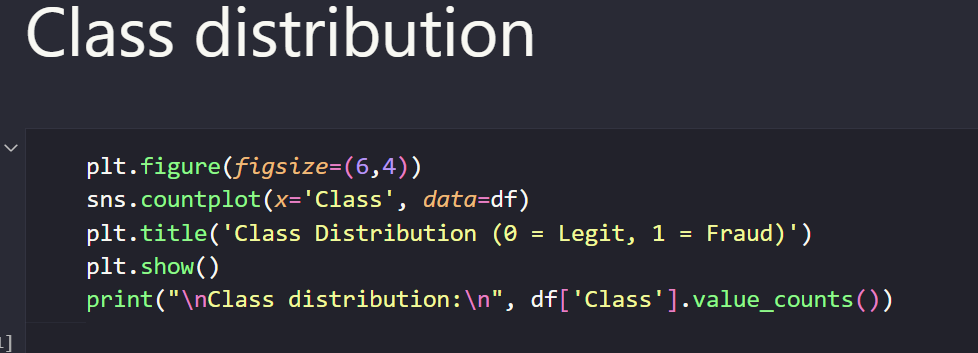
\includegraphics[width=1.00\linewidth]{images/image_p19_3.png}
\end{figure}

\begin{figure}[H]
\centering
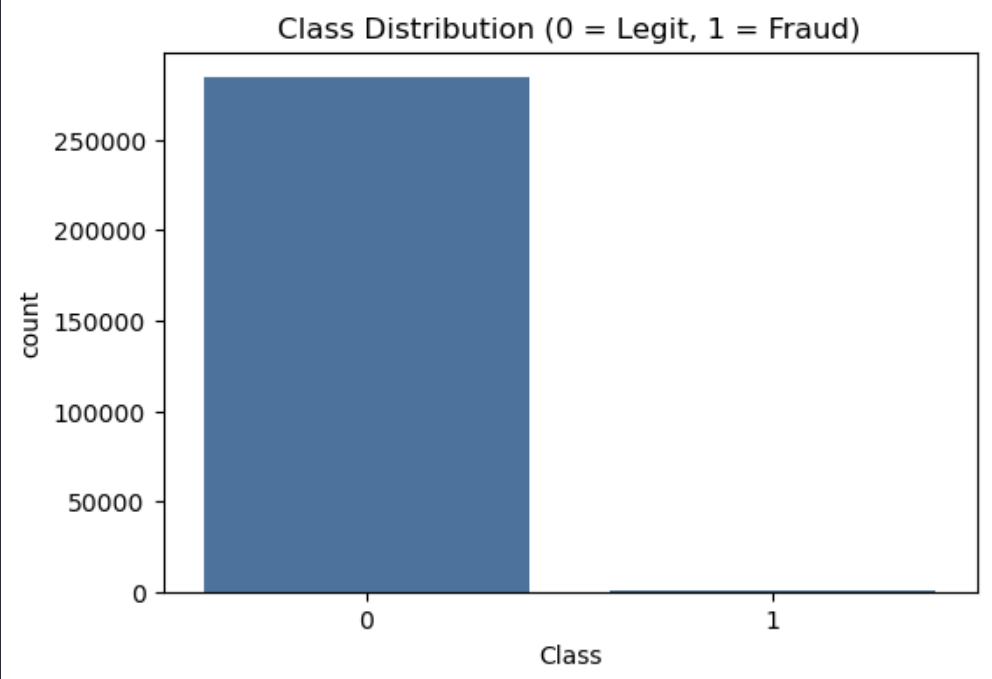
\includegraphics[width=1.00\linewidth]{images/image_p19_4.png}
\end{figure}

Page | 18  

\newpage

\begin{figure}[H]
\centering
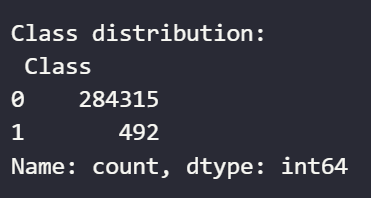
\includegraphics[width=0.74\linewidth]{images/image_p20_5.png}
\end{figure}

\begin{figure}[H]
\centering
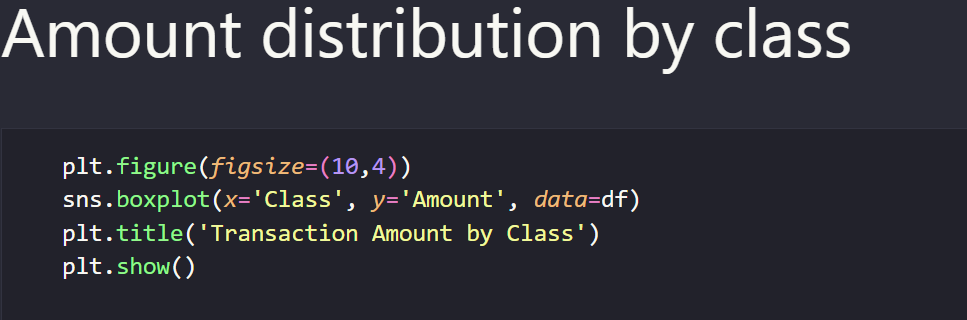
\includegraphics[width=1.00\linewidth]{images/image_p20_6.png}
\end{figure}

\subsection*{2 Amount Distribution by class: }

Page | 19  

\newpage

\begin{figure}[H]
\centering
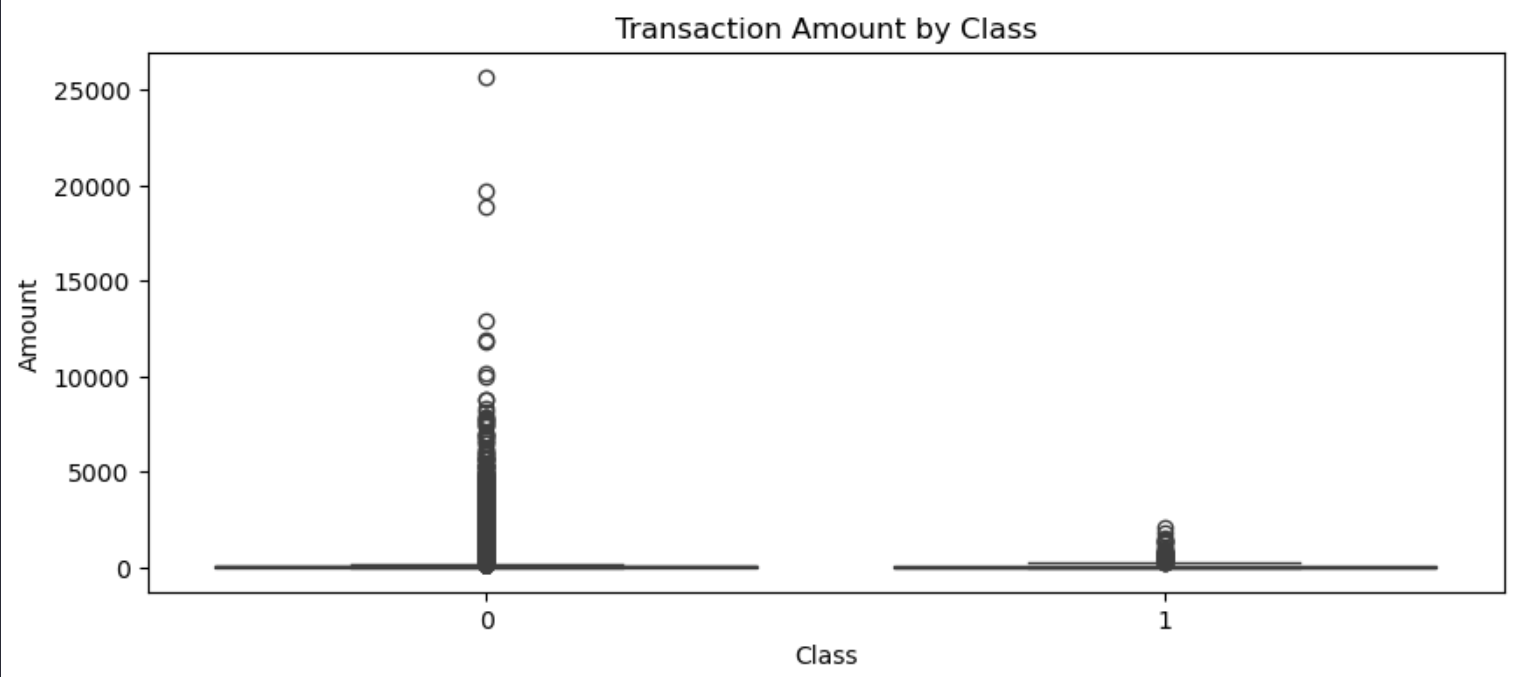
\includegraphics[width=1.00\linewidth]{images/image_p21_7.png}
\end{figure}

\begin{figure}[H]
\centering
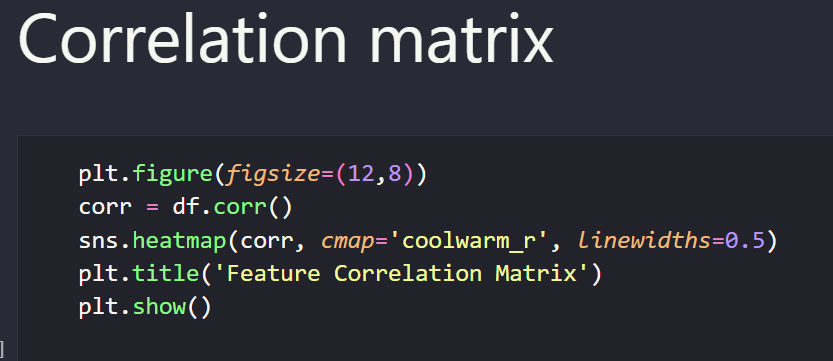
\includegraphics[width=1.00\linewidth]{images/image_p21_8.png}
\end{figure}

\subsection*{3 Correlation matrix: }

Page | 20  

\newpage

\begin{figure}[H]
\centering
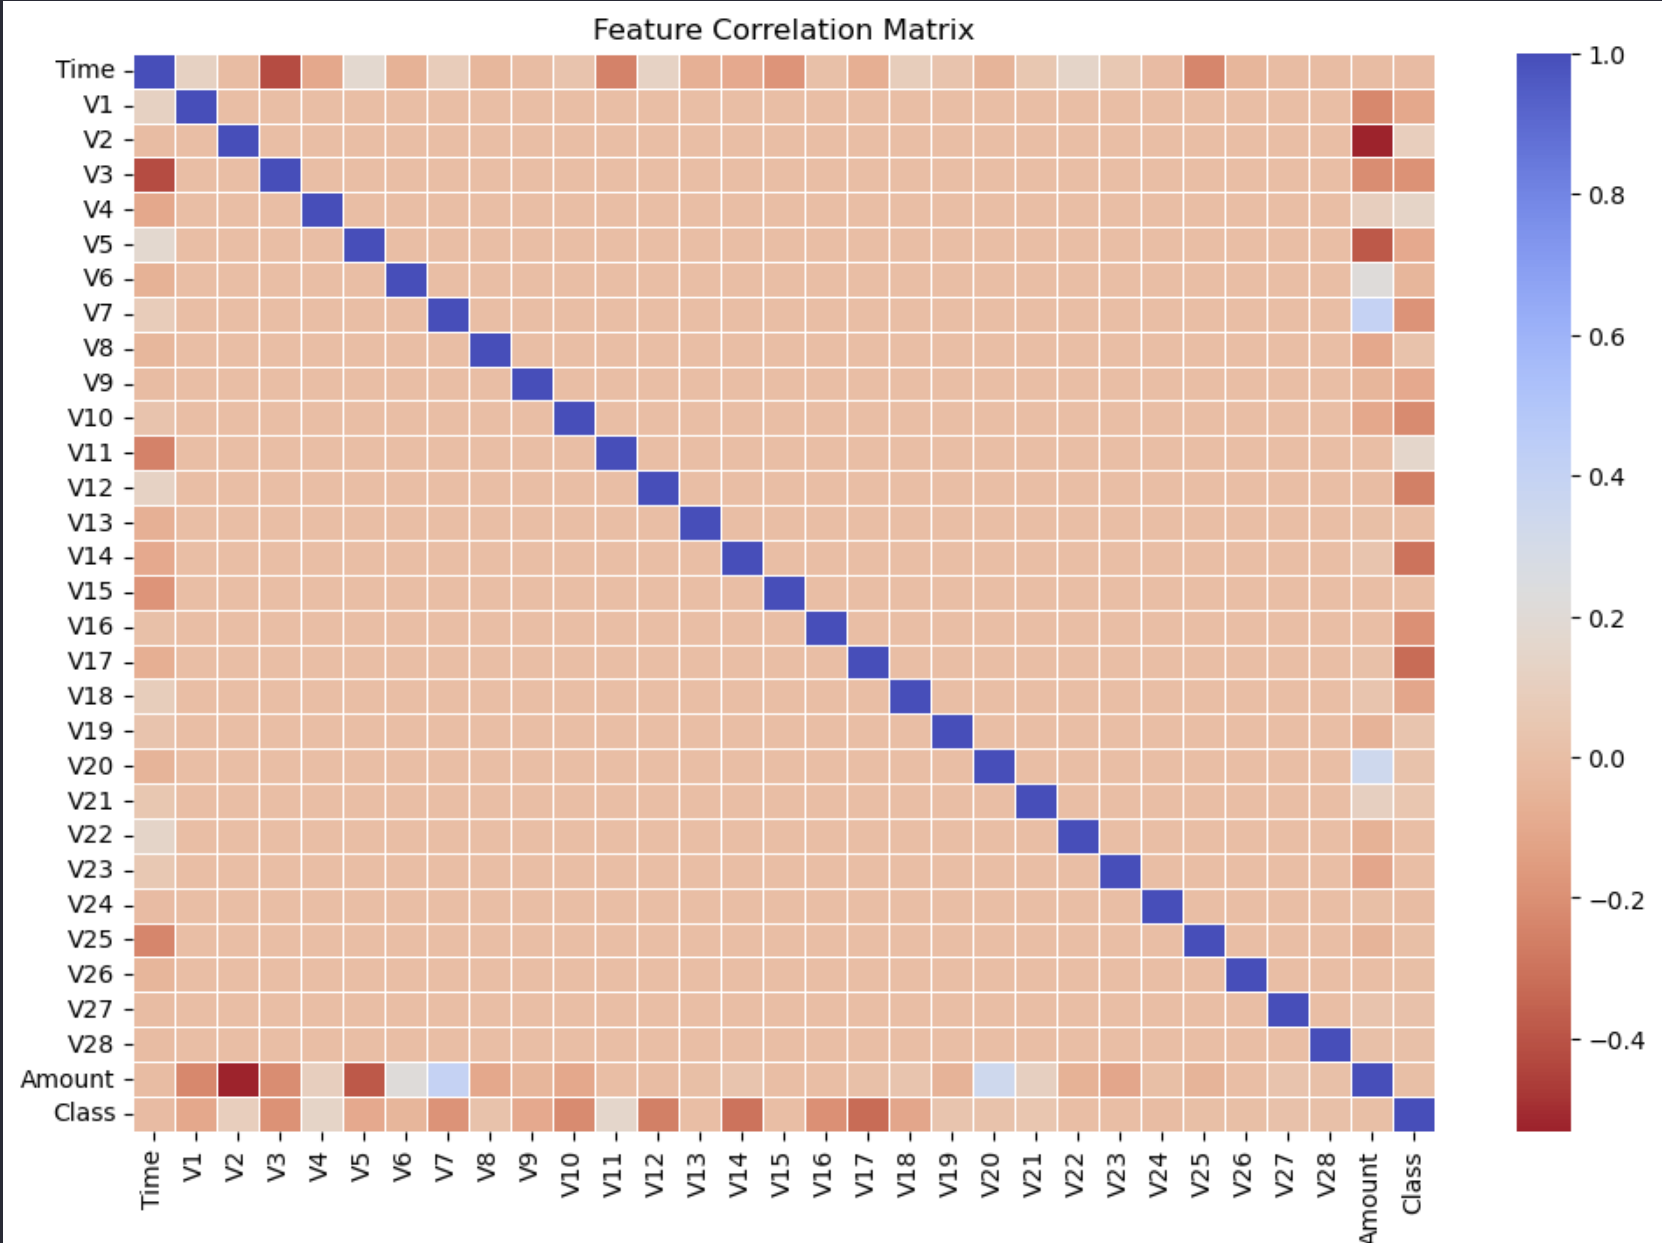
\includegraphics[width=1.00\linewidth]{images/image_p22_9.png}
\end{figure}

\begin{figure}[H]
\centering
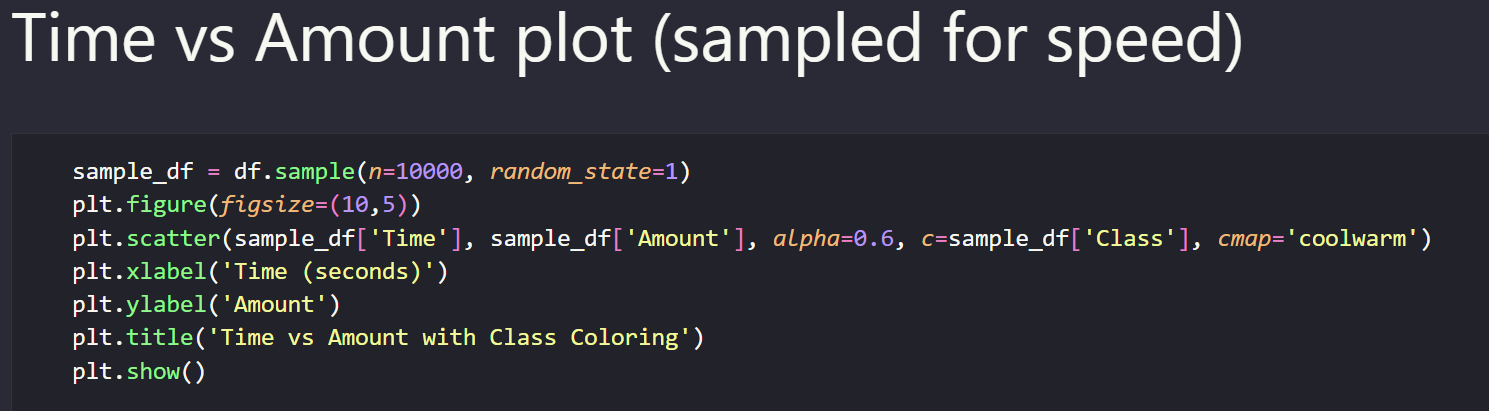
\includegraphics[width=1.00\linewidth]{images/image_p22_10.png}
\end{figure}

\subsection*{4 Time vs Amount plot: }

Page | 21  

\newpage

\begin{figure}[H]
\centering
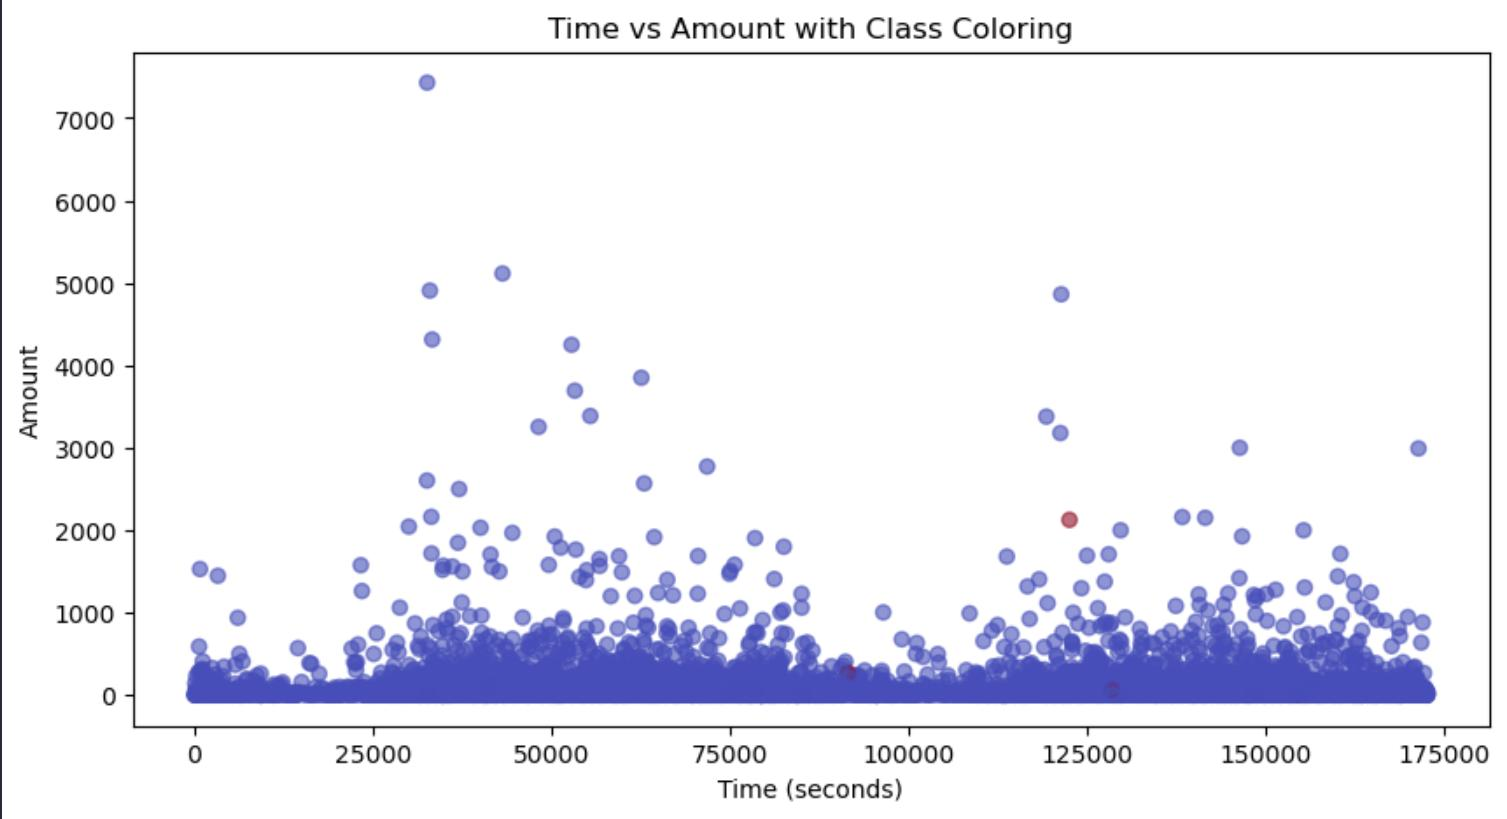
\includegraphics[width=1.00\linewidth]{images/image_p23_11.jpeg}
\end{figure}

\begin{figure}[H]
\centering
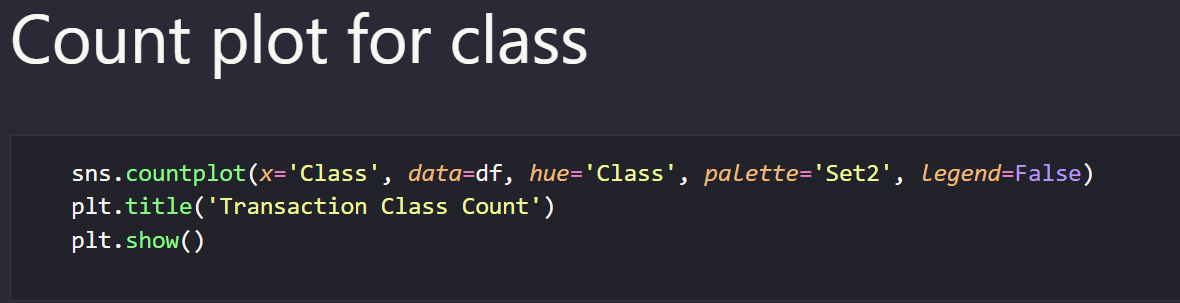
\includegraphics[width=1.00\linewidth]{images/image_p23_12.png}
\end{figure}

\subsection*{5. Count plot for class: }

Page | 22  

\newpage

\begin{figure}[H]
\centering
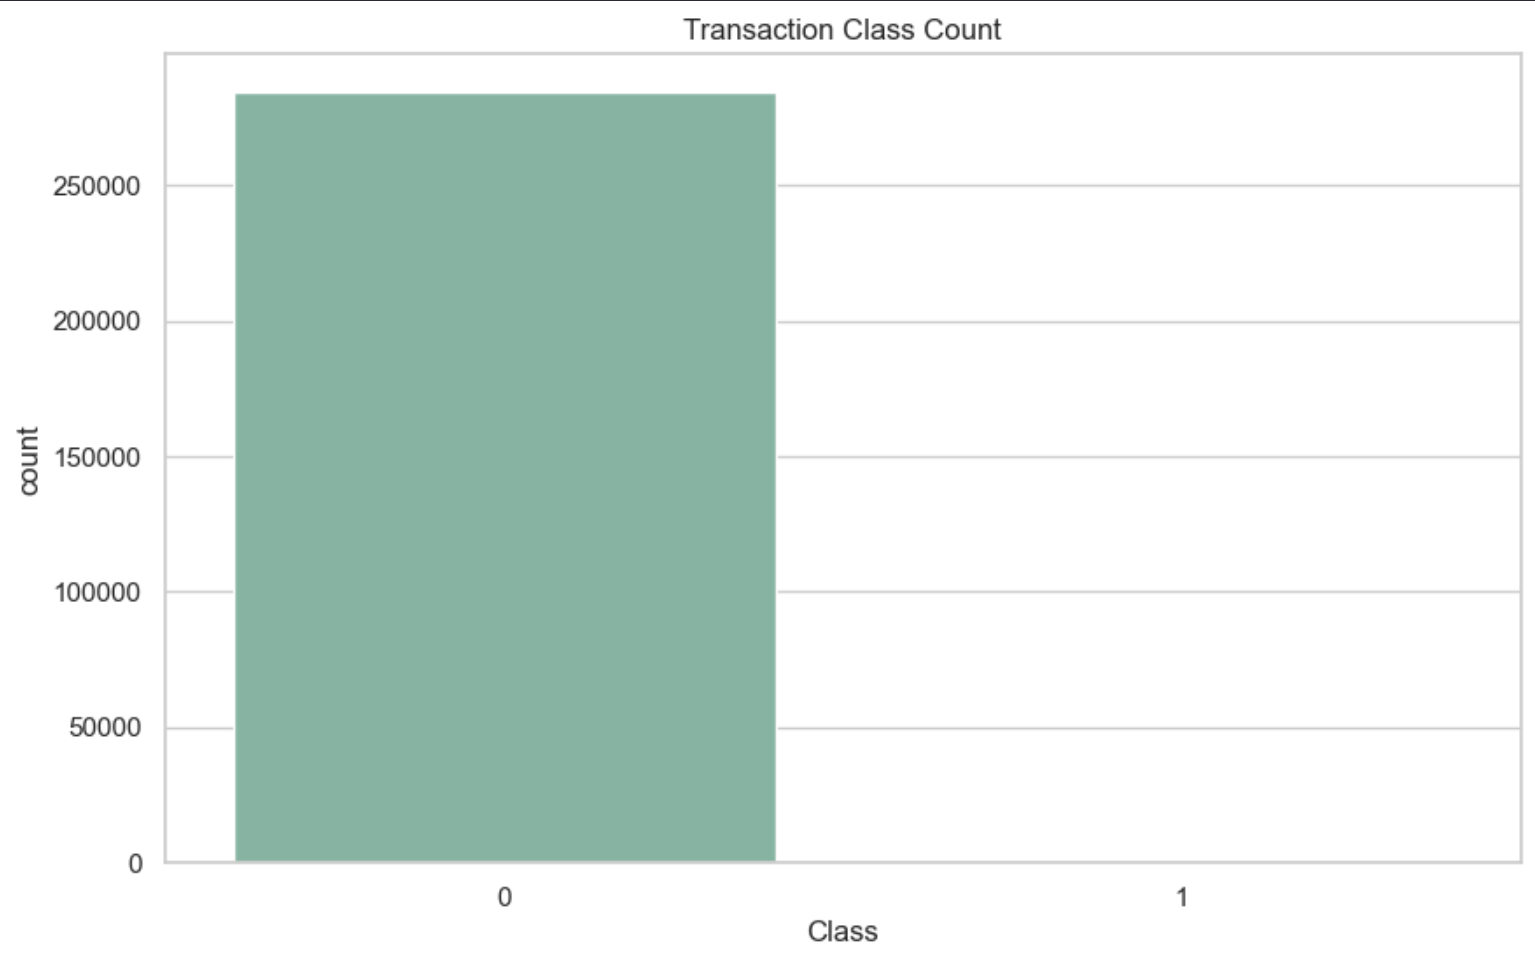
\includegraphics[width=1.00\linewidth]{images/image_p24_13.png}
\end{figure}

\begin{figure}[H]
\centering
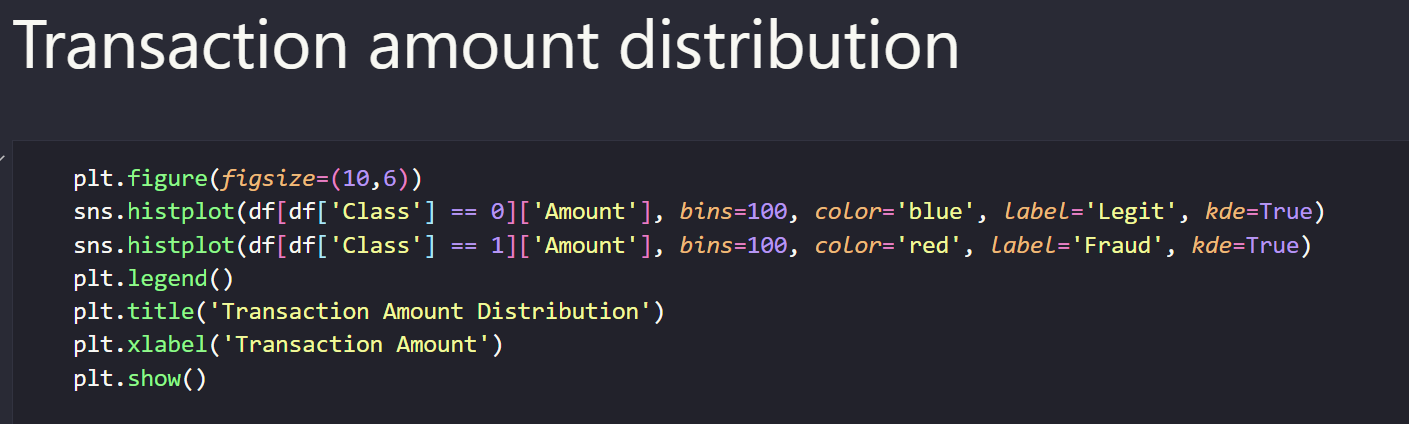
\includegraphics[width=1.00\linewidth]{images/image_p24_14.png}
\end{figure}

\subsection*{6. Transaction amount distribution: }

Page | 23  

\newpage

\begin{figure}[H]
\centering
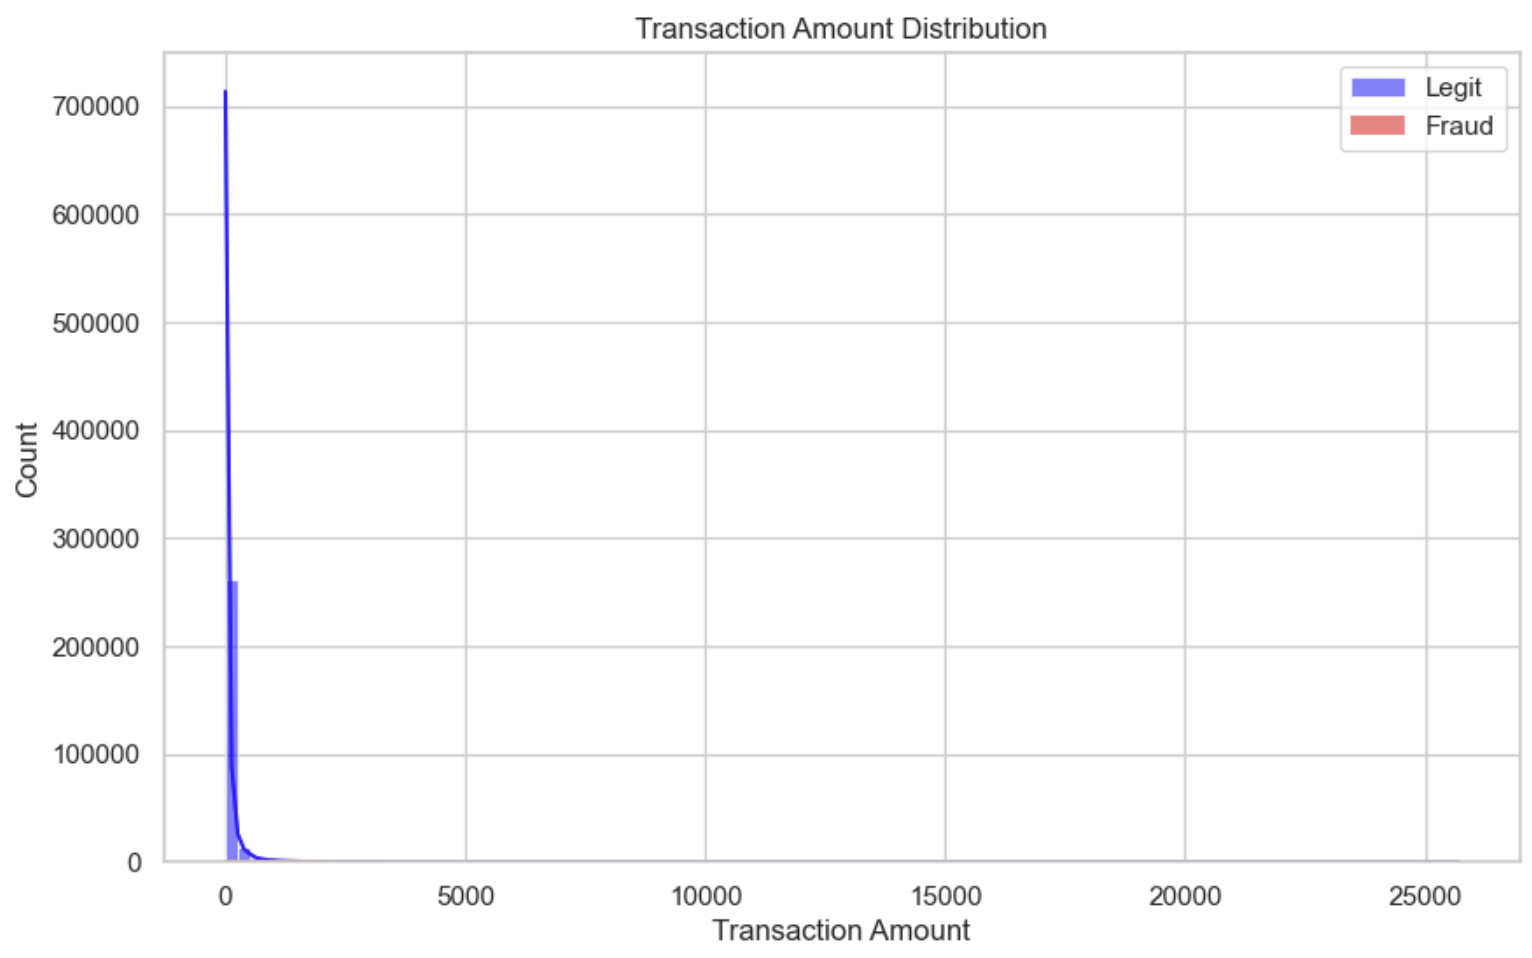
\includegraphics[width=1.00\linewidth]{images/image_p25_15.png}
\end{figure}

\begin{figure}[H]
\centering
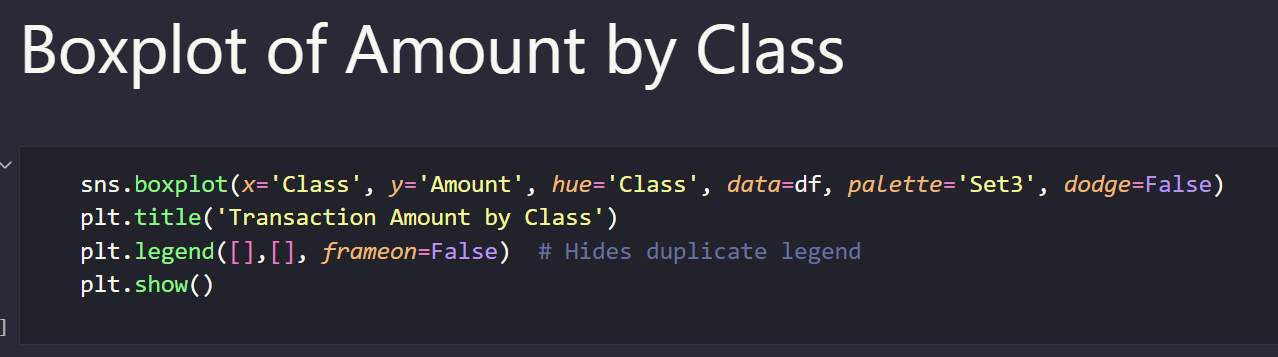
\includegraphics[width=1.00\linewidth]{images/image_p25_16.png}
\end{figure}

\subsection*{7. Boxplot of Amount by class: }

Page | 24  

\newpage

\begin{figure}[H]
\centering
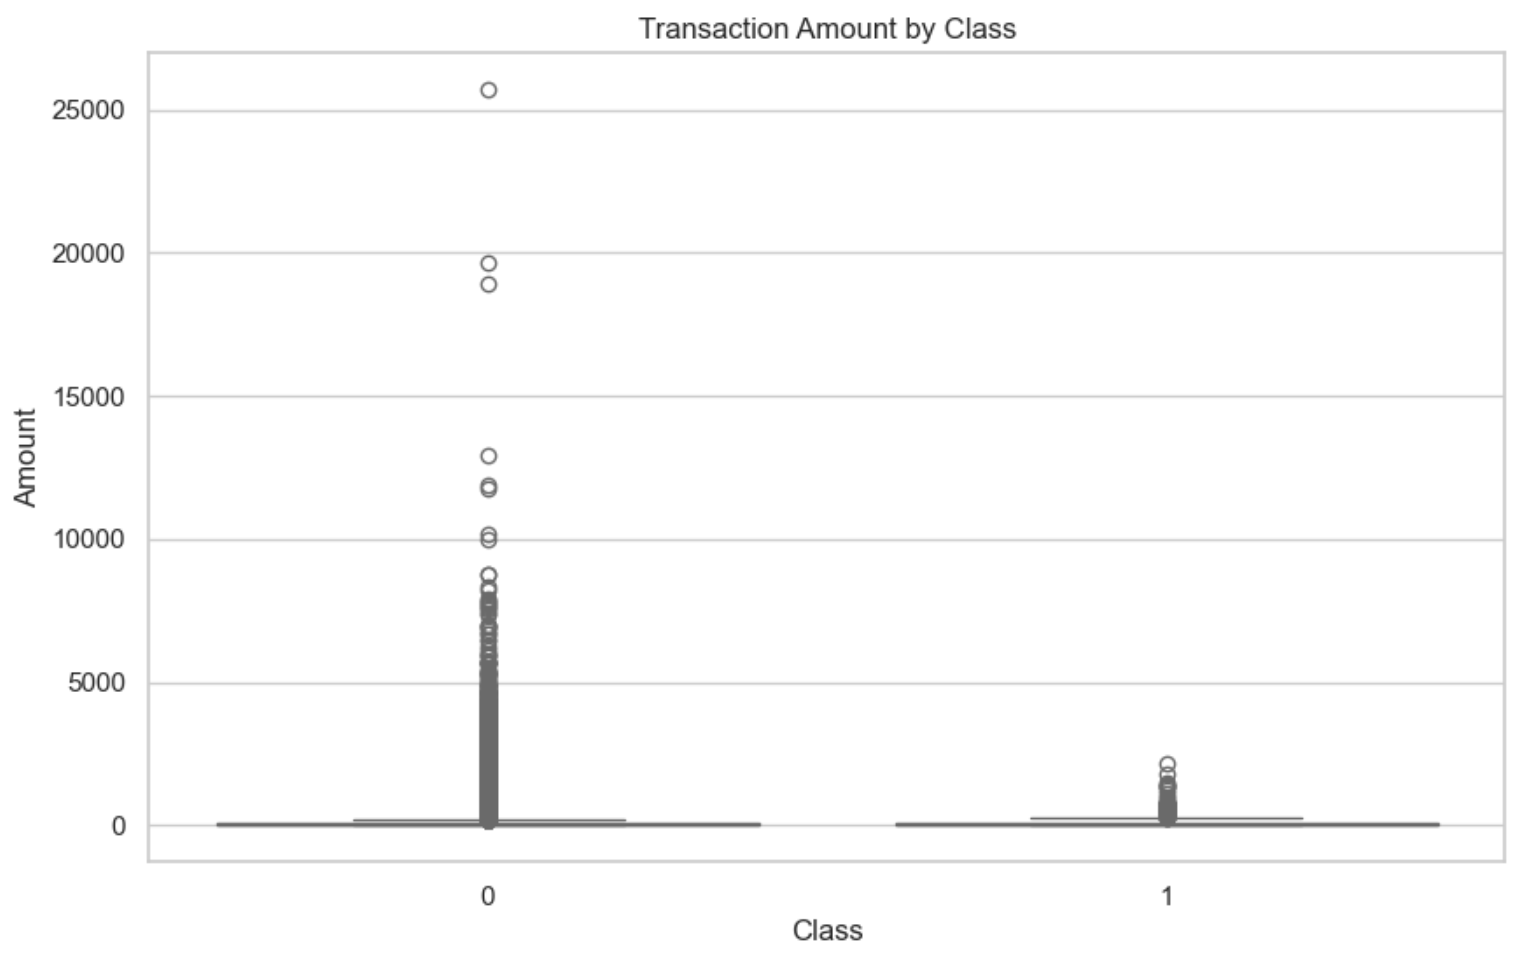
\includegraphics[width=1.00\linewidth]{images/image_p26_17.png}
\end{figure}

\begin{figure}[H]
\centering
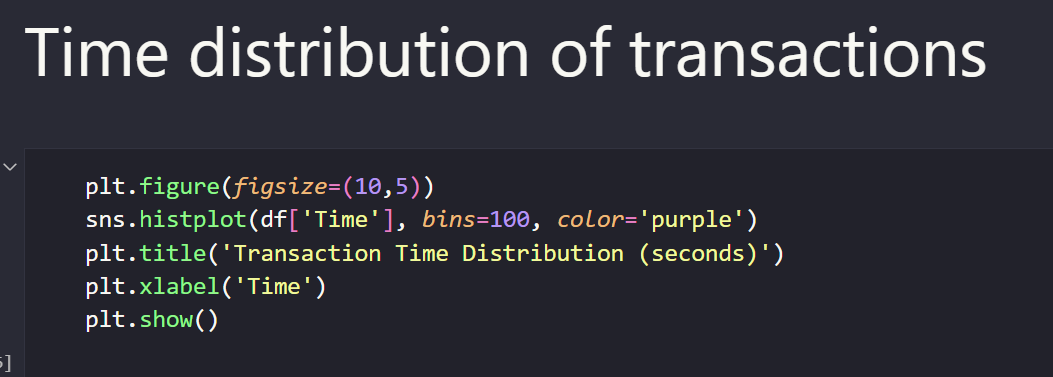
\includegraphics[width=1.00\linewidth]{images/image_p26_18.png}
\end{figure}

\subsection*{ 8. Time distribution of transactions: }

Page | 25  

\newpage

\begin{figure}[H]
\centering
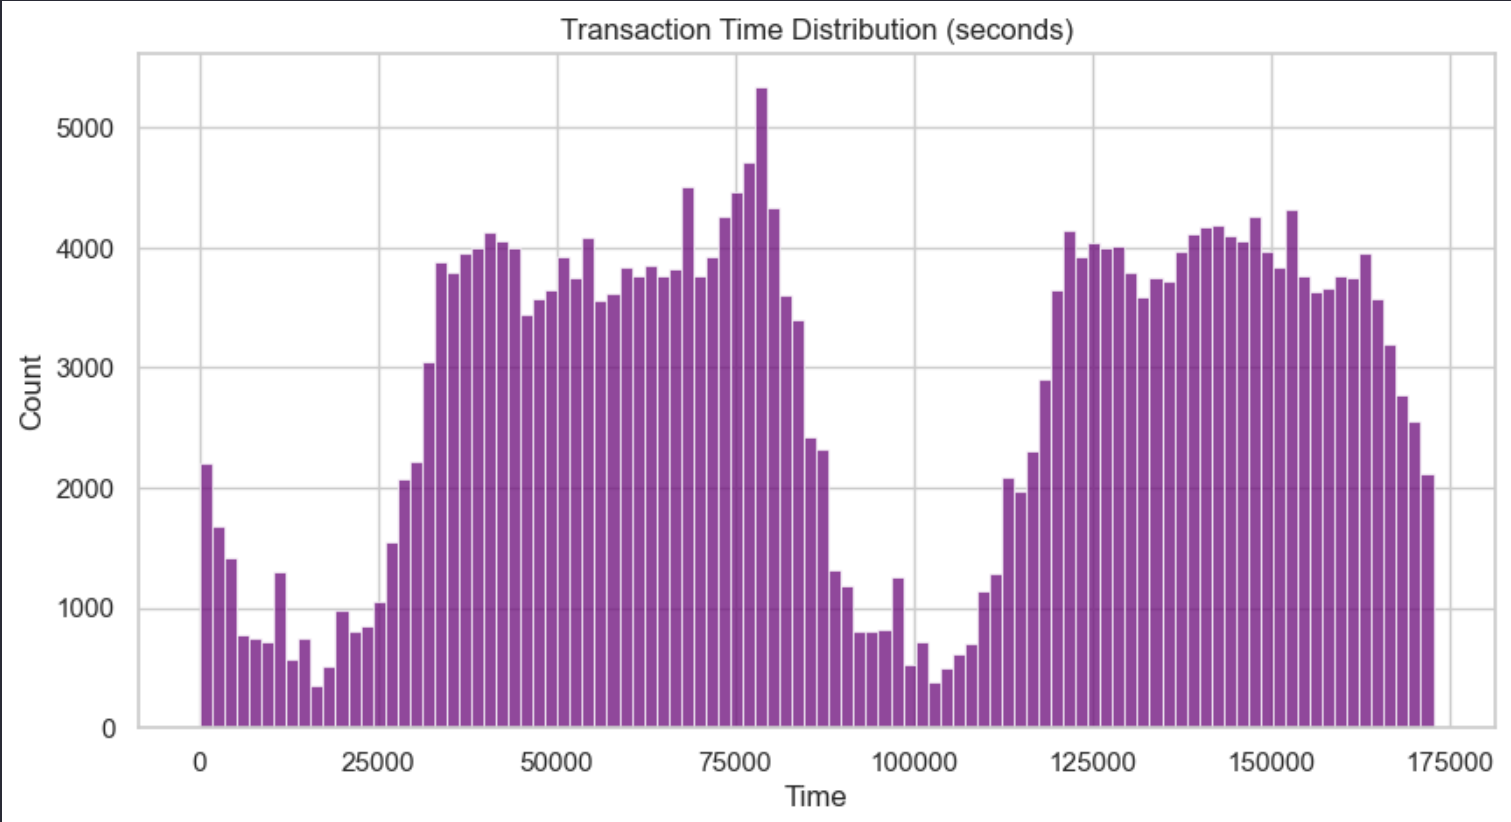
\includegraphics[width=1.00\linewidth]{images/image_p27_19.png}
\end{figure}

\begin{figure}[H]
\centering
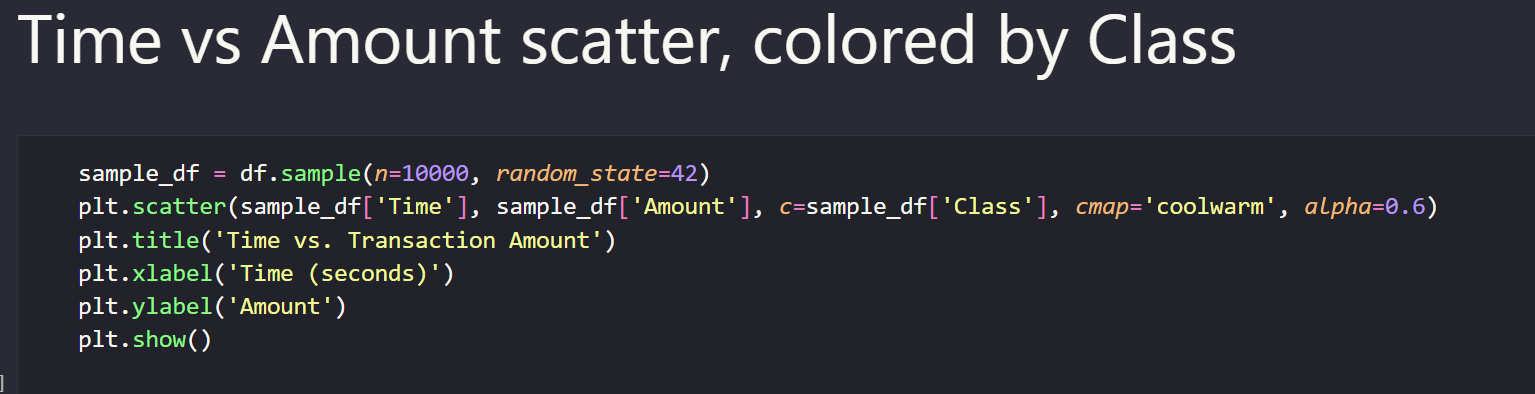
\includegraphics[width=1.00\linewidth]{images/image_p27_20.png}
\end{figure}

\subsection*{9. Time vs Amount scatter, colored by class: }

Page | 26  

\newpage

\begin{figure}[H]
\centering
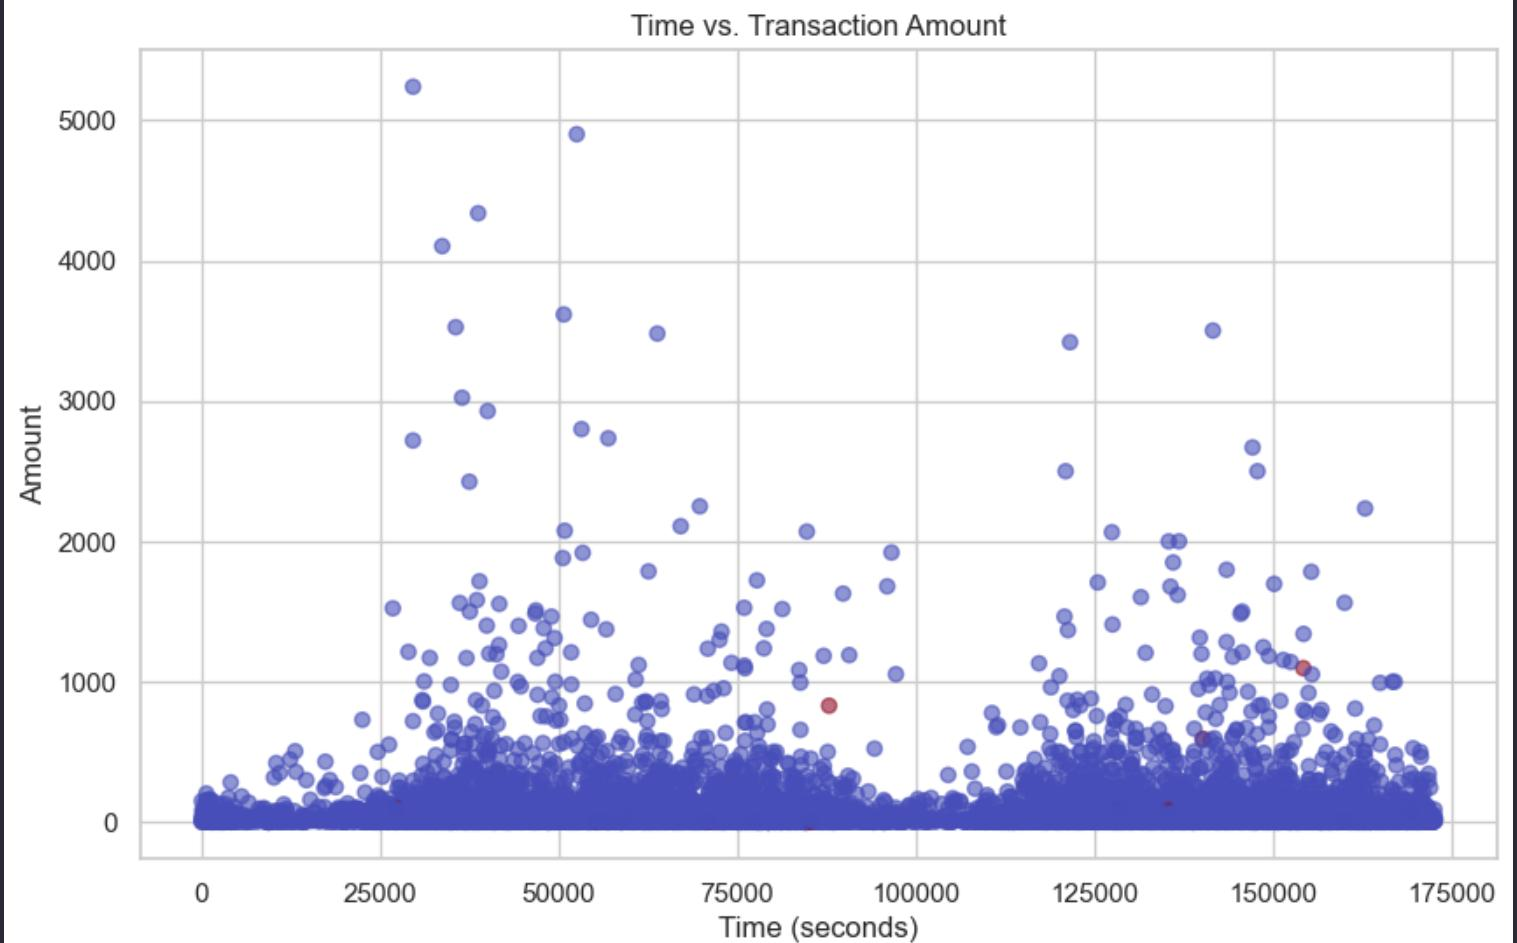
\includegraphics[width=1.00\linewidth]{images/image_p28_21.jpeg}
\end{figure}

\begin{figure}[H]
\centering
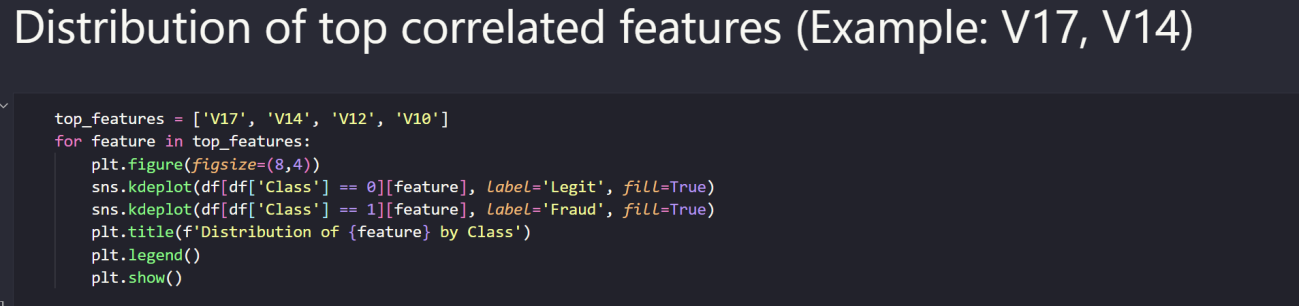
\includegraphics[width=1.00\linewidth]{images/image_p28_22.png}
\end{figure}

\subsection*{10. Distribution of top correlated features: }

Page | 27  

\newpage

\begin{figure}[H]
\centering
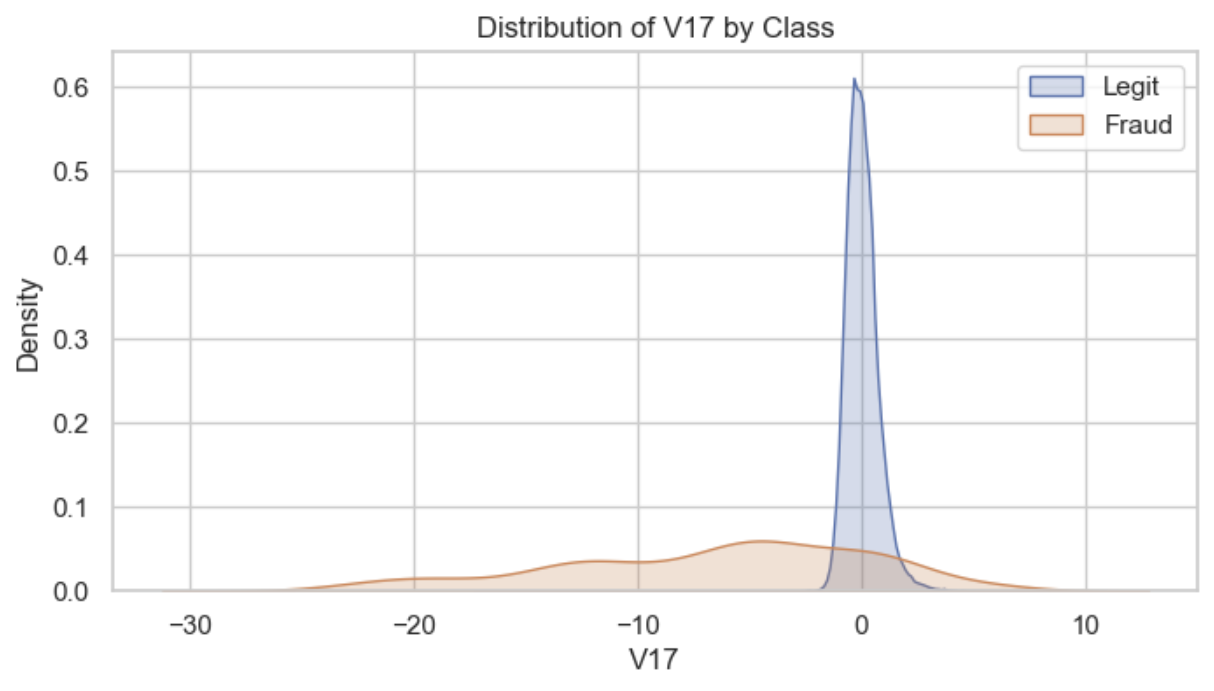
\includegraphics[width=1.00\linewidth]{images/image_p29_23.png}
\end{figure}

\begin{figure}[H]
\centering
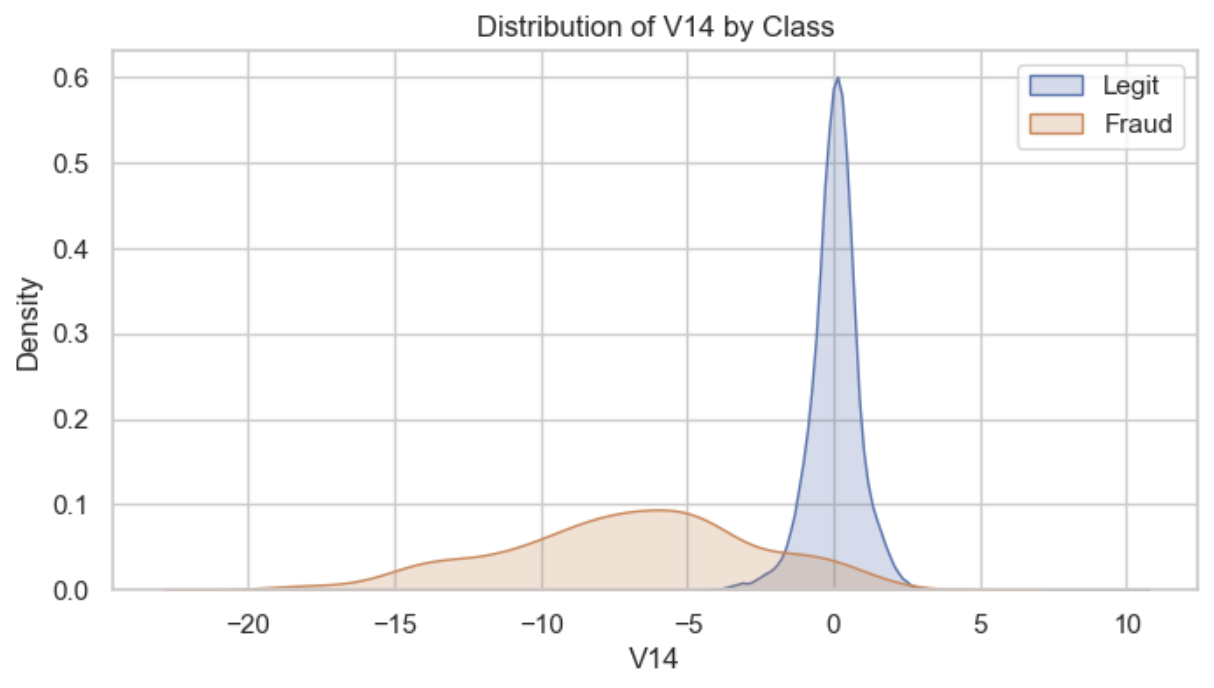
\includegraphics[width=1.00\linewidth]{images/image_p29_24.png}
\end{figure}

Page | 28  

\newpage

\begin{figure}[H]
\centering
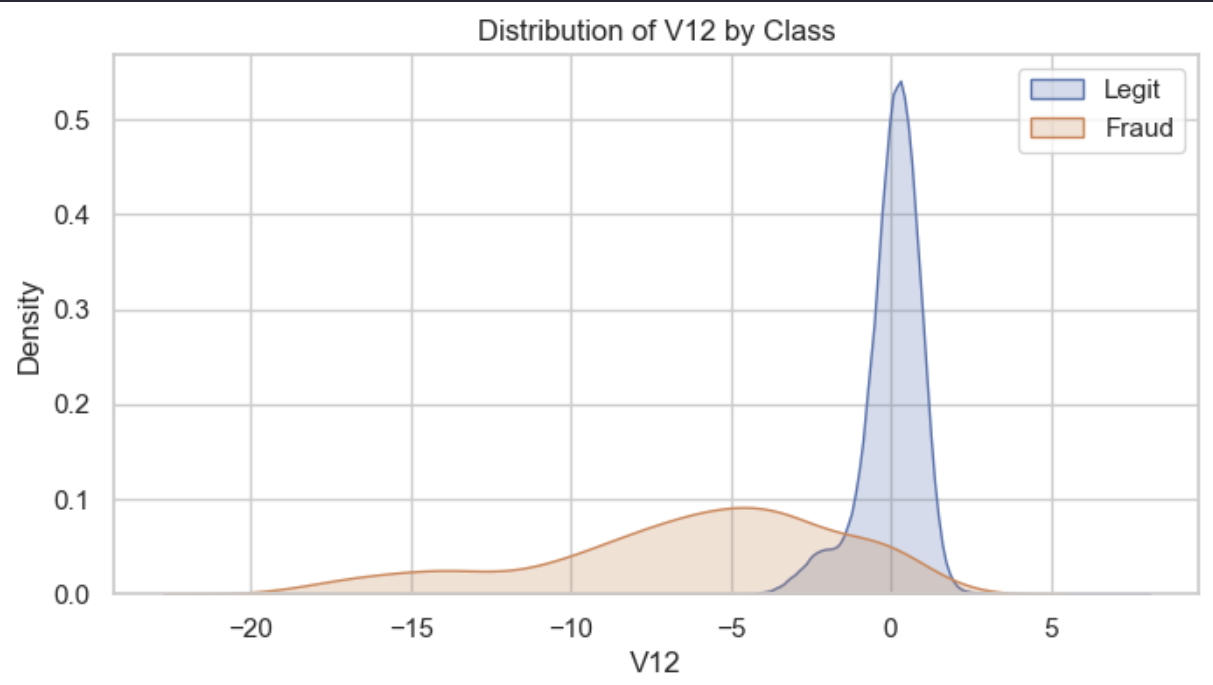
\includegraphics[width=1.00\linewidth]{images/image_p30_25.png}
\end{figure}

\begin{figure}[H]
\centering
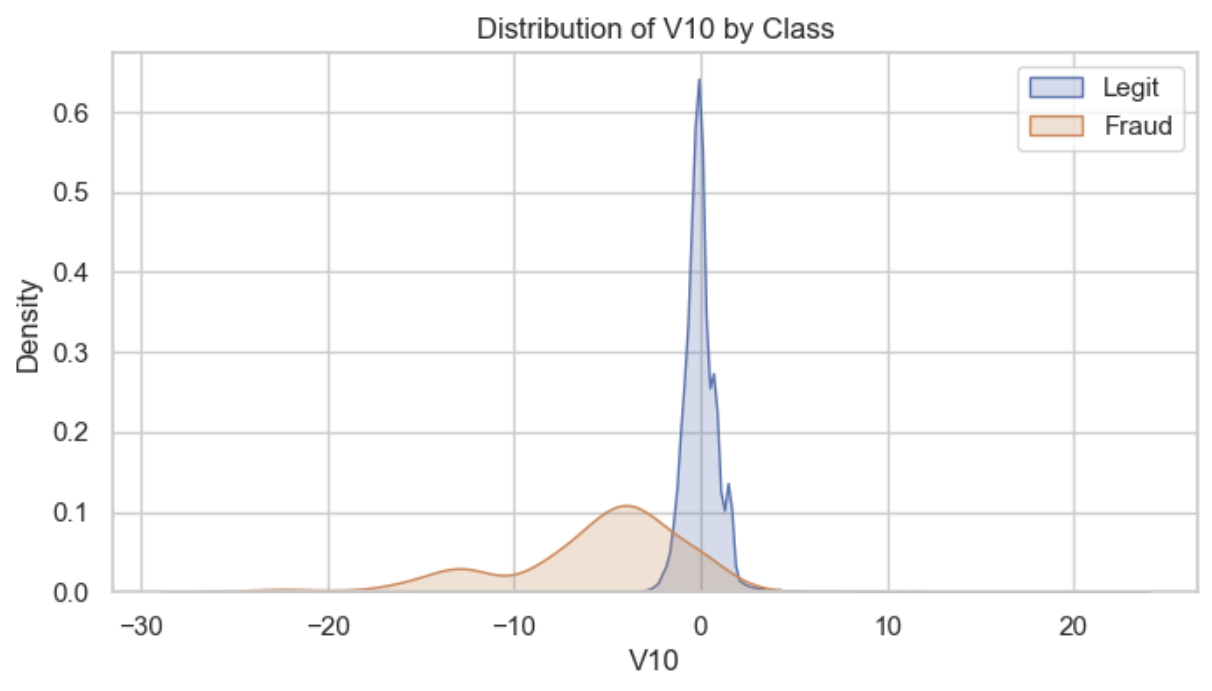
\includegraphics[width=1.00\linewidth]{images/image_p30_26.png}
\end{figure}

\begin{figure}[H]
\centering
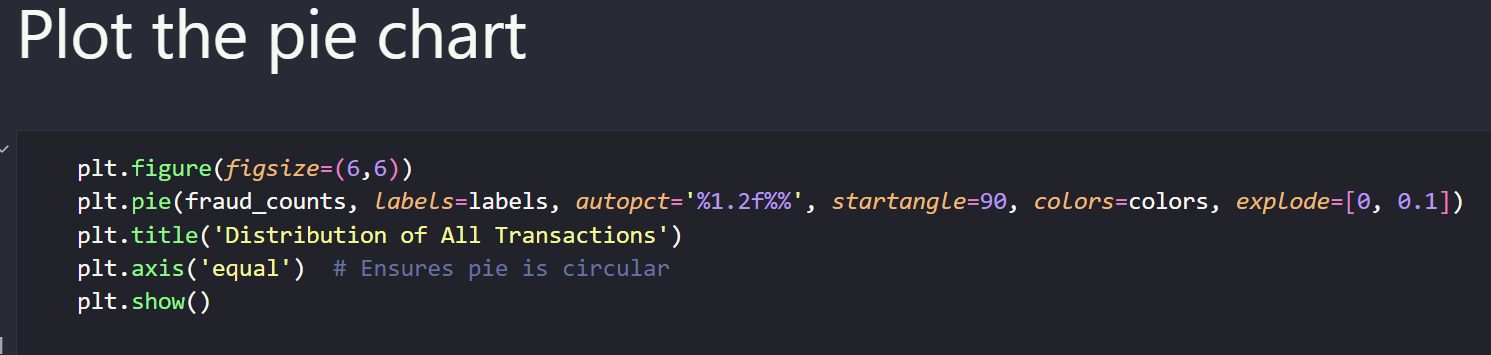
\includegraphics[width=1.00\linewidth]{images/image_p30_27.png}
\end{figure}

\subsection*{11. plot the pie chart: }

Page | 29  

\newpage

\begin{figure}[H]
\centering
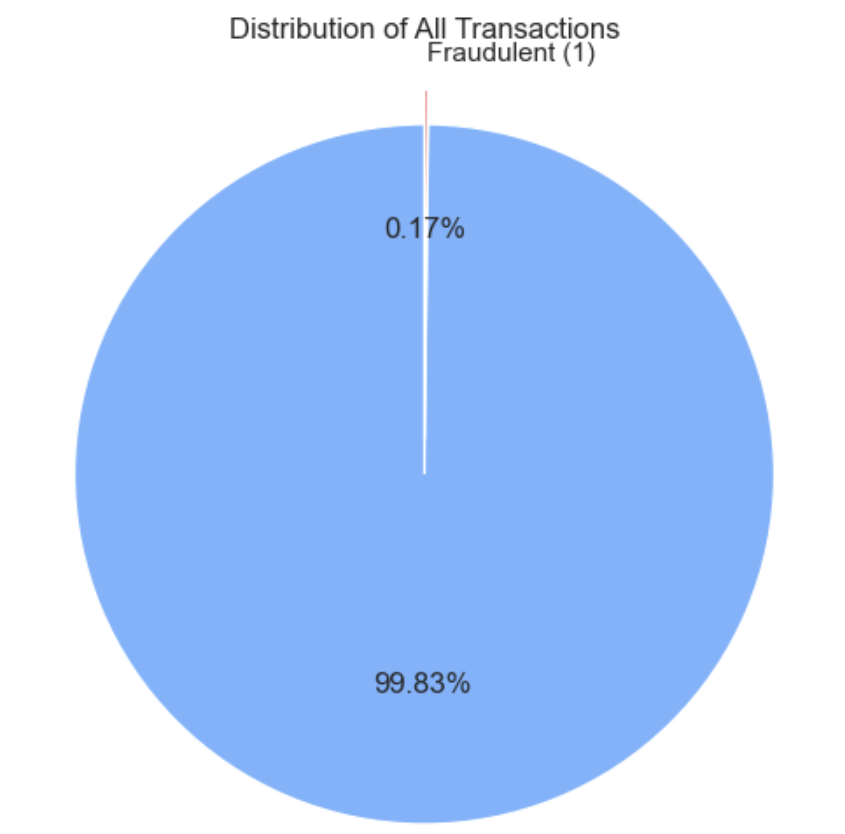
\includegraphics[width=1.00\linewidth]{images/image_p31_28.png}
\end{figure}

\begin{figure}[H]
\centering
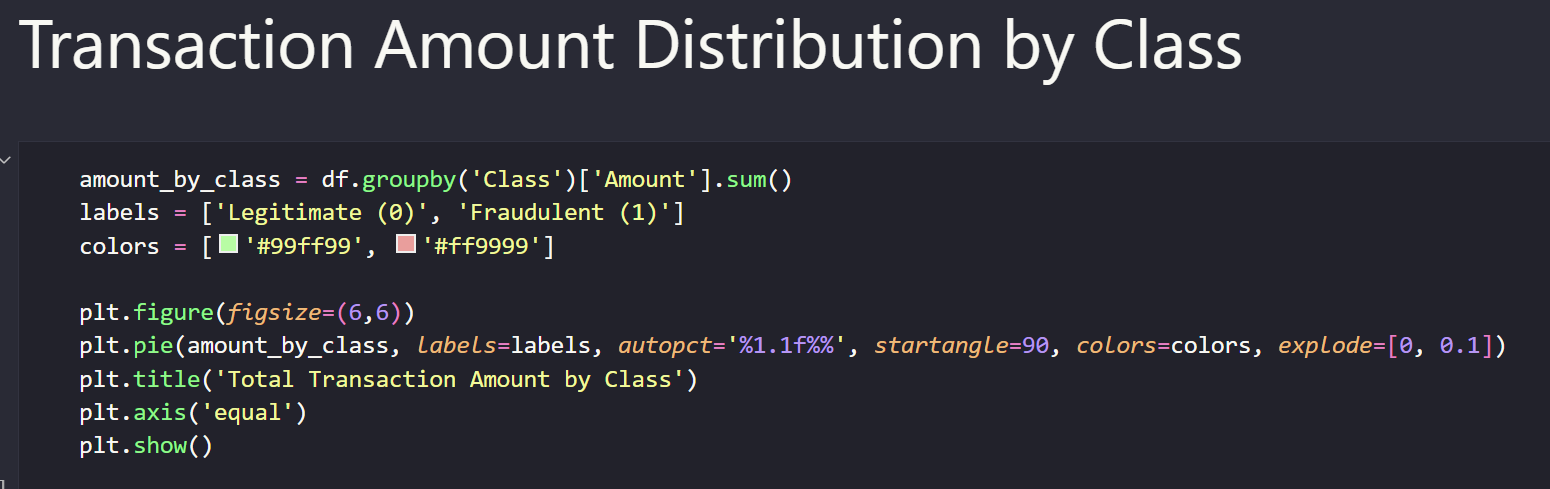
\includegraphics[width=1.00\linewidth]{images/image_p31_29.png}
\end{figure}

Page | 30  

\newpage

\begin{figure}[H]
\centering
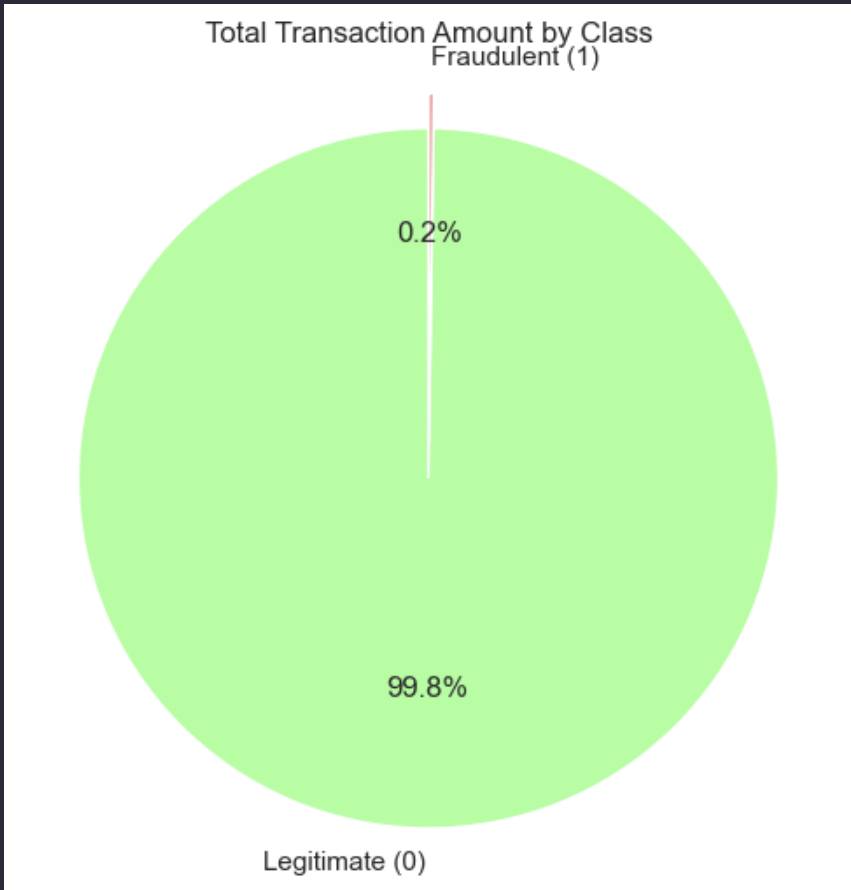
\includegraphics[width=1.00\linewidth]{images/image_p32_30.png}
\end{figure}

Page | 31  

\newpage

\begin{figure}[H]
\centering
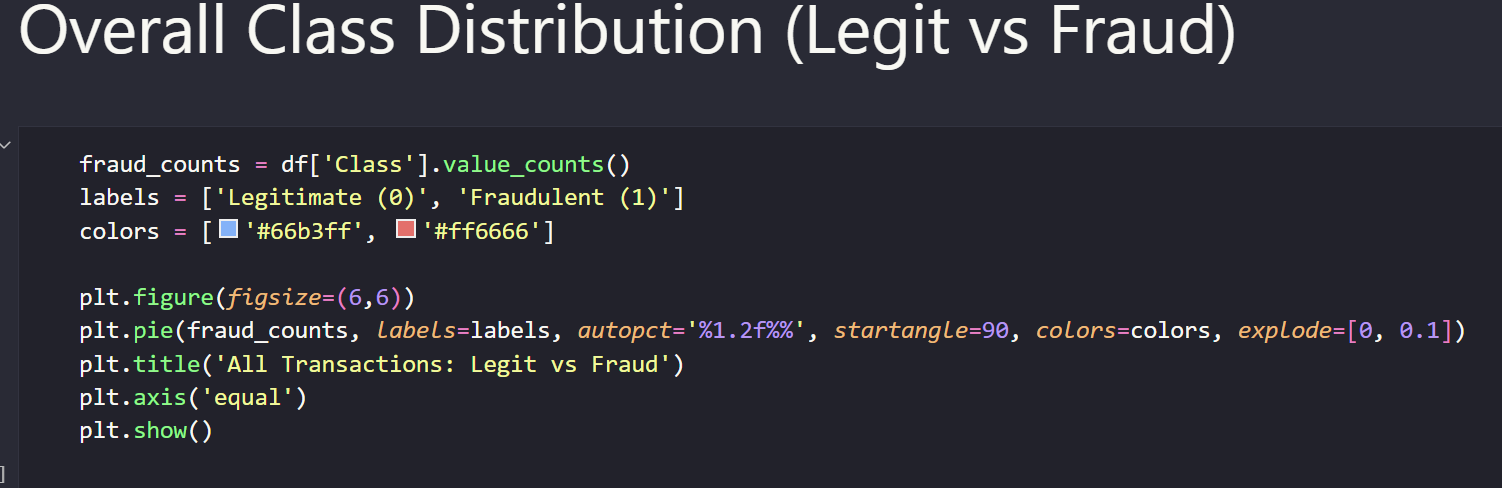
\includegraphics[width=1.00\linewidth]{images/image_p33_31.png}
\end{figure}

\begin{figure}[H]
\centering
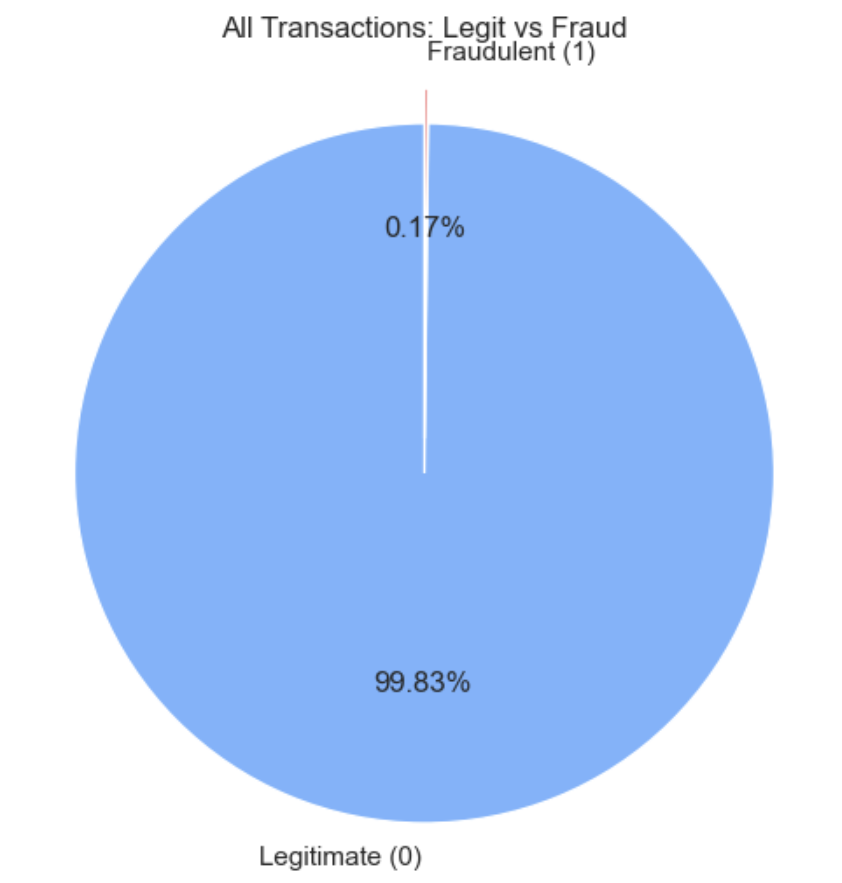
\includegraphics[width=1.00\linewidth]{images/image_p33_32.png}
\end{figure}

Page | 32  

\newpage

\begin{figure}[H]
\centering
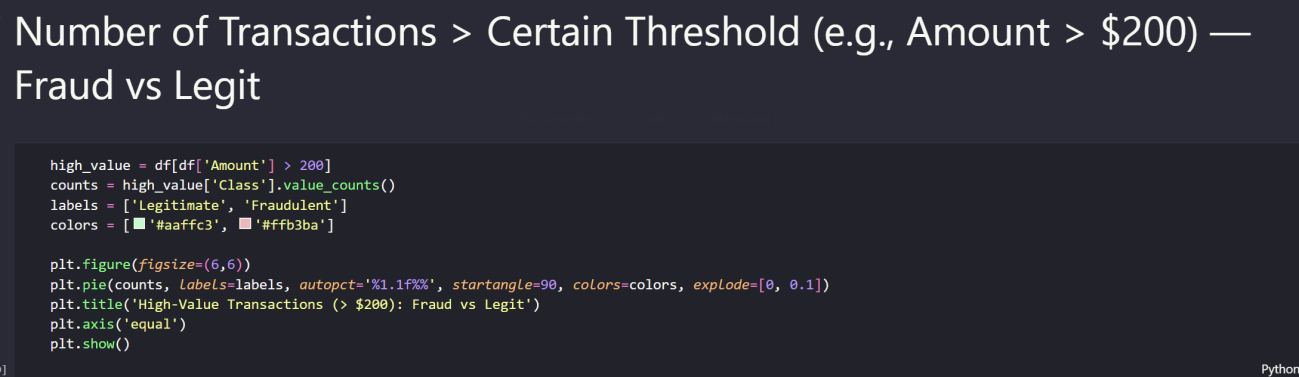
\includegraphics[width=1.00\linewidth]{images/image_p34_33.png}
\end{figure}

\begin{figure}[H]
\centering
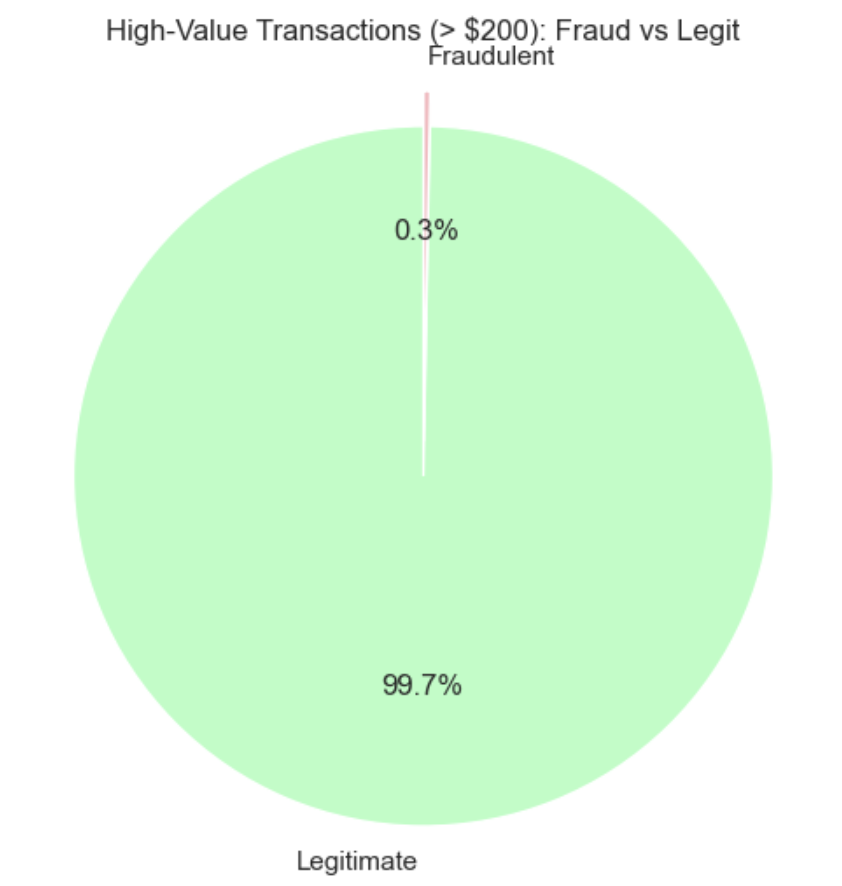
\includegraphics[width=1.00\linewidth]{images/image_p34_34.png}
\end{figure}

\subsection*{12. Fraud Distribution by Hour: }

Page | 33  

\newpage

\begin{figure}[H]
\centering
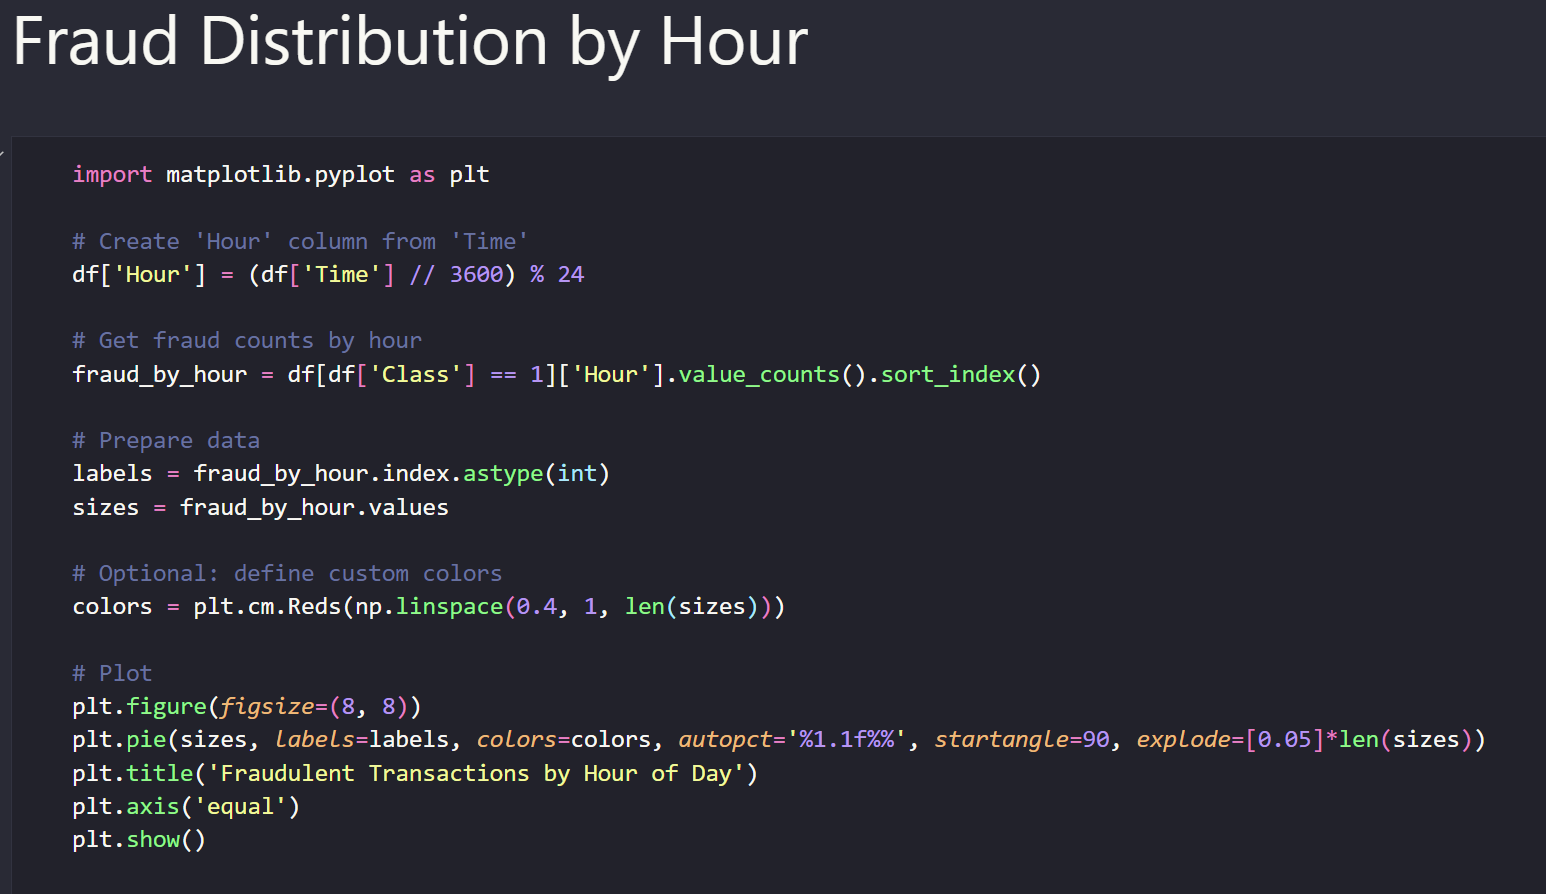
\includegraphics[width=1.00\linewidth]{images/image_p35_35.png}
\end{figure}

\begin{figure}[H]
\centering
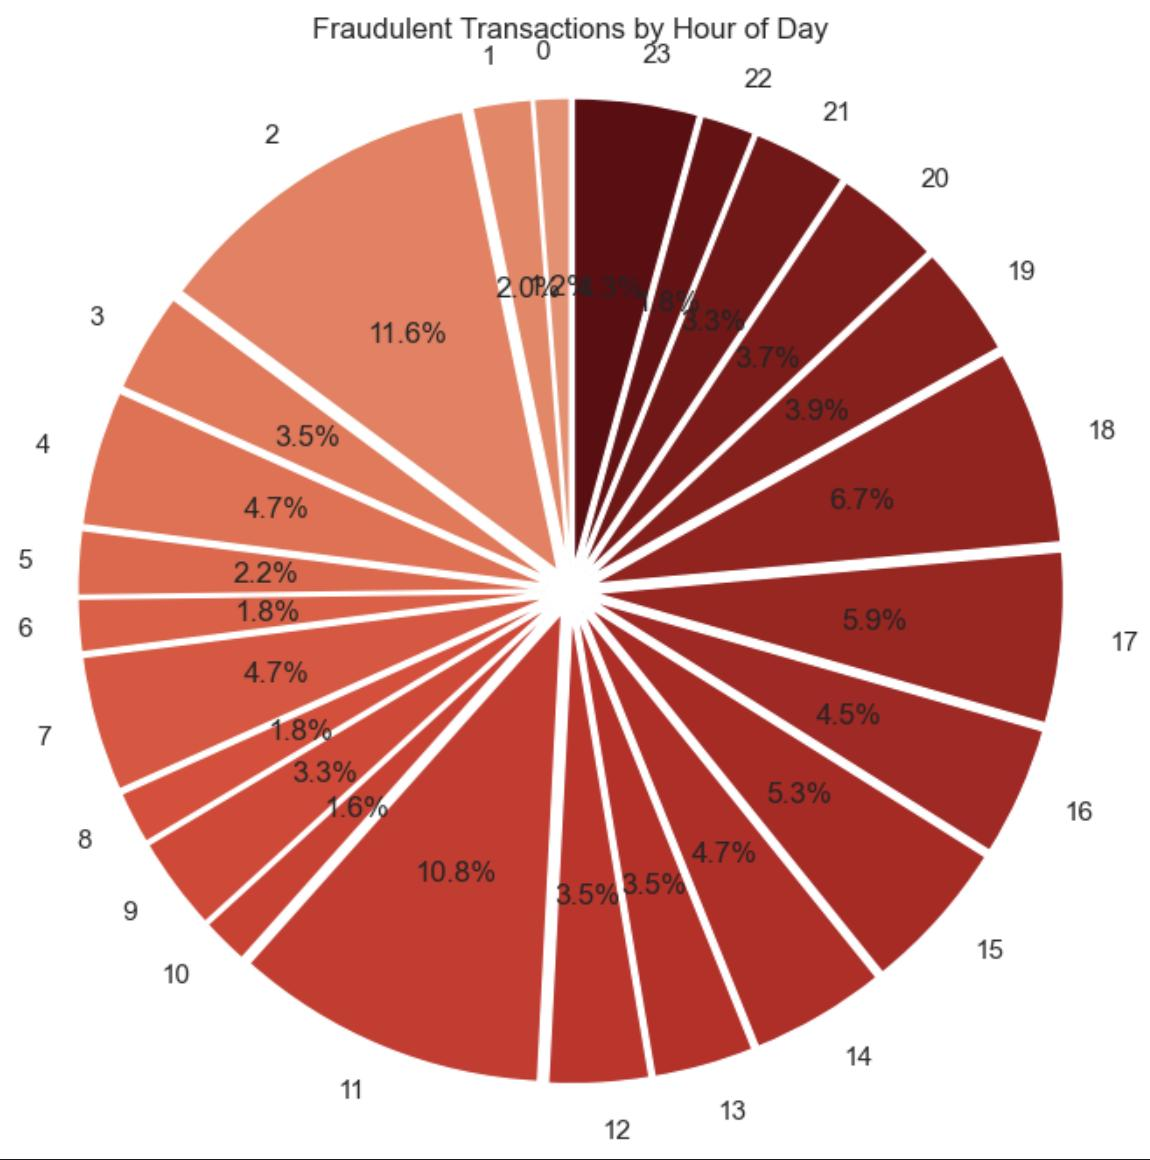
\includegraphics[width=1.00\linewidth]{images/image_p35_36.jpeg}
\end{figure}

Page | 34  

\newpage

\subsection*{3. SYSTEM IMPLIMENTATION DETAILS }

This section details the step-by-step implementation of the Credit Card Fraud Detection System, 

elaborating on the applied methodology, technology stack, and essential source code 
integrations. 

\subsubsection*{3.1 Methodology Adopted }

To ensure accuracy and adaptability in fraud detection, the project applies a structured, data-

driven machine learning methodology. The approach is modular, ensuring that each 
component—from preprocessing to deployment—can be individually developed, tested, and 
maintained. Below are the primary stages involved: 

1. Data Collection: The Kaggle Credit Card Fraud Detection dataset is utilized, which 

contains anonymized features derived through PCA, along with 'Time', 'Amount', and a 
'Class' label. 

\subsubsection*{2. Preprocessing: }

o Feature Scaling: Time and Amount are normalized using StandardScaler to ensure 

uniformity. 

o Class Balancing: The dataset’s high imbalance (fraud cases <1\%) is handled using 

\begin{center}
SMOTE, which synthetically creates samples of the minority class. 
\end{center}

\subsubsection*{3. Model Training: }

\begin{center}
o A RandomForestClassifier is selected for its accuracy and robustness. 
\end{center}

o The model is trained using a stratified train-test split to preserve class distribution. 

o The trained model is saved using joblib for deployment. 

\subsubsection*{4. Model Evaluation: }

o Accuracy alone is not sufficient; thus, evaluation metrics such as F1-score, Recall, 

Precision, and ROC-AUC are used. 

o Confusion matrix and ROC curve visualizations help validate the model's 

performance on imbalanced data. 

\subsubsection*{5. Model Deployment: }

\begin{center}
o Streamlit, a Python-based UI framework, is used to deploy the model. 
\end{center}

o A responsive and simple interface allows users to manually input transaction 

attributes. 

\subsubsection*{6. Real-Time Prediction: }

o Upon user input, the deployed model returns a fraud prediction and a corresponding 

confidence score. 

o The feedback is immediately displayed via Streamlit, mimicking a real-time 

prediction system. 

This methodology ensures modularity, extensibility, and real-time inference—all critical for a 

fraud detection application. 

Page | 35  

\newpage

\subsubsection*{3.2 Hardware and Software Used }

To effectively build and test the application, specific hardware and software resources were used 

as listed below. 

\subsubsection*{Hardware Requirements: }

• 
Processor: Intel i5 / AMD Ryzen 5 or higher 

• 
RAM: Minimum 8 GB (recommended for faster training) 

• 
Storage: At least 2 GB of free space 

• 
Operating System: Windows 10 or Linux (Ubuntu 20.04 tested) 

\subsubsection*{Software Requirements: }

• 
Programming Language: Python 3.8 or higher 

• 
Key Libraries: 

o pandas, numpy: Data manipulation 

o scikit-learn: Model building and evaluation 

o imblearn: SMOTE oversampling 

o joblib: Model serialization 

o matplotlib, seaborn: Visualization 

o streamlit: Web interface for real-time predictions 

• 
Development Tools: 

\begin{center}
o Visual Studio Code / Jupyter Notebook (for coding and testing) 
\end{center}

o Git (for version control) 

• 
Browser: Chrome / Firefox (to test Streamlit interface) 

This setup allows the entire project to be built and tested locally without requiring advanced GPU 

support. 

\subsubsection*{3.3 Summary }

This implementation strategically combines real-world data, appropriate machine learning 

techniques, and web interface design. Each component—from preprocessing to prediction—
is modular, scalable, and well-documented. The use of SMOTE addresses class imbalance, 
while Streamlit enhances usability by offering an interactive fraud prediction interface. 

The system reflects modern software engineering and data science best practices, making it 

suitable for both academic demonstration and as a foundational prototype for real-world 
fraud detection solutions. The implementation strategy successfully combines machine 
learning, software modularity, and real-time interactivity. Each script and component has 
been designed for extensibility, making the system ideal for both academic learning and 
future production-scale fraud detection systems. 

Page | 36  

\newpage

\section*{4. DESIGN }

This section outlines the architectural and structural design of the Credit Card Fraud Detection 
System. It includes the system flowchart to illustrate the operational logic and an Entity 
Relationship Diagram (ERD) to depict the data flow and interdependencies between major system 
components. 

\subsubsection*{4.1 Flowchart }

The flowchart represents the logical flow of the system from data loading to final prediction 
display. It provides a step-by-step structure of how the backend processes interact and how the user 
interfaces with the fraud detection model. 

Flow Steps: 

1. Start: System is initialized. 

2. Load Dataset: The creditcard.csv file is loaded using pandas. 

\subsubsection*{3. Data Preprocessing: }

o Scale the Time and Amount fields using StandardScaler. 

o Apply SMOTE to synthetically balance the dataset. 

\subsubsection*{4. Model Training: }

o The RandomForestClassifier is trained on the preprocessed and resampled dataset. 

\subsubsection*{5. Evaluation: }

o The model is evaluated using classification metrics (Accuracy, Precision, Recall, F1-

Score, ROC-AUC). 

o Confusion matrix and ROC curve are generated. 

\subsubsection*{6. Model Saving: }

o The trained model is saved using joblib. 

\subsubsection*{7. UI Interaction: }

o The Streamlit interface is launched. 

\begin{center}
o User inputs transaction details (features V1–V28, Amount). 
\end{center}

\subsubsection*{8. Prediction: }

o The model predicts whether the transaction is fraudulent or legitimate. 

o The result and confidence score are displayed. 

Page | 37  

\newpage

\begin{figure}[H]
\centering
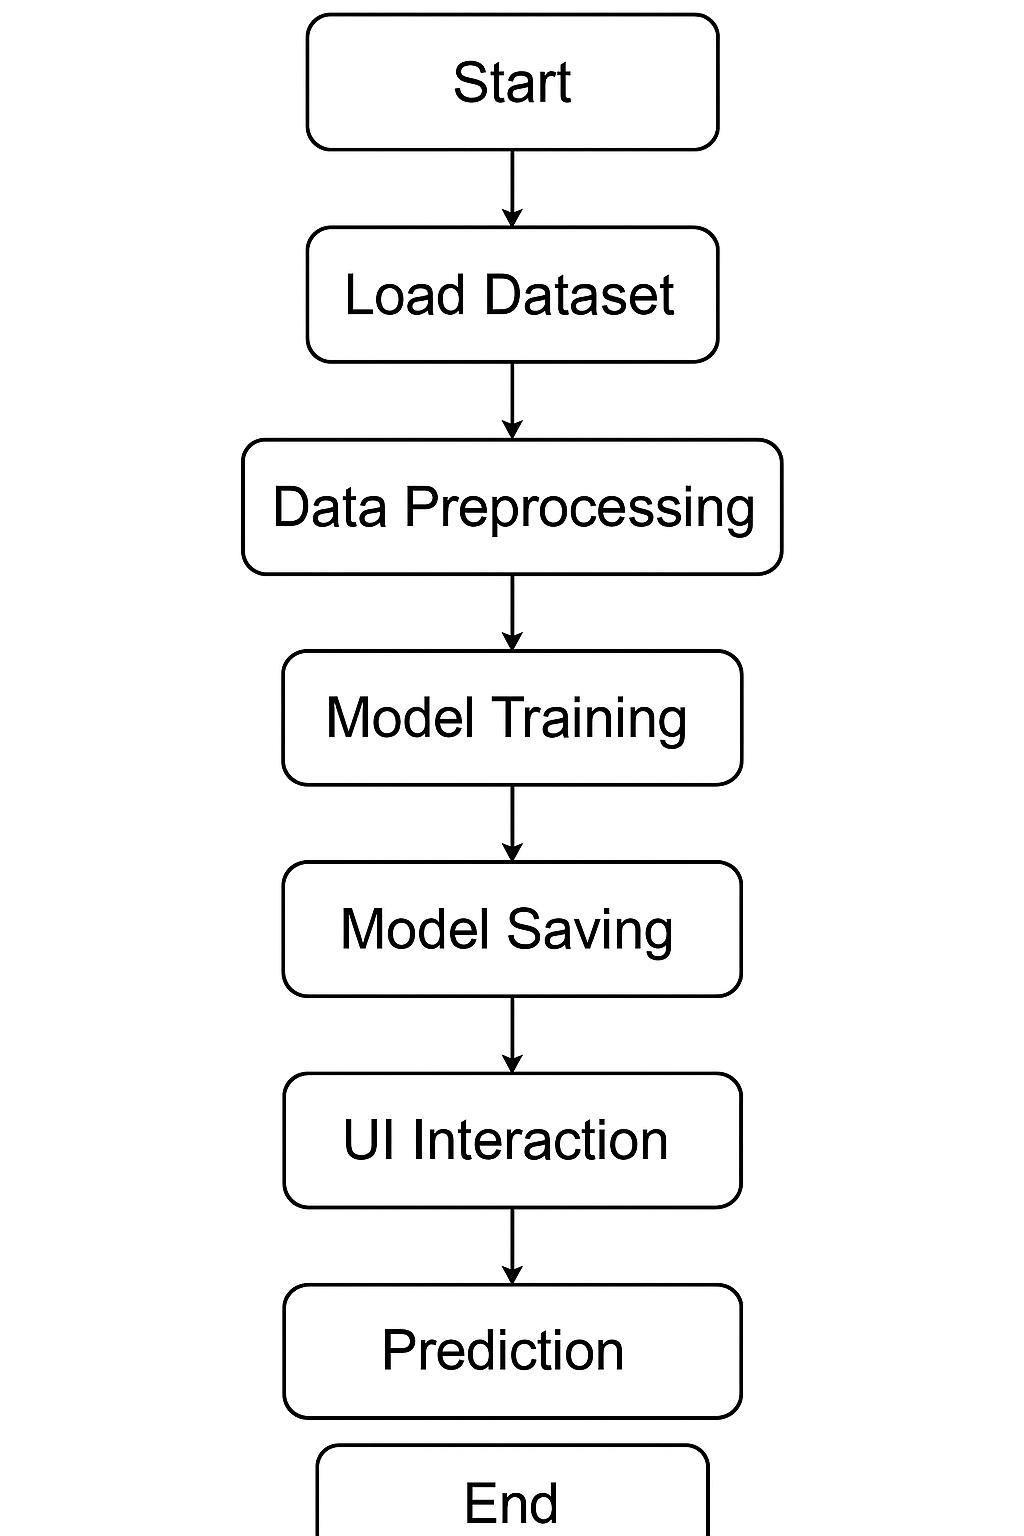
\includegraphics[width=1.00\linewidth]{images/image_p39_37.jpeg}
\end{figure}

9. End: The system awaits further inputs or closes. 

Flowchart: 

This flow ensures that each component is tightly integrated but independently testable, maintaining 
robustness and flexibility. 

\subsubsection*{7.2 Entity Relationship Diagram (ERD) }

The ERD defines how different entities within the system relate to each other, particularly in terms 
of data attributes and model interactions. Each entity represents a logical component or process 
within the fraud detection system. 

Entities and Attributes: 

Page | 38  

\newpage

\subsubsection*{1. Transaction: }

o Transaction\_ID (PK) 

o Time 

o Amount 

o Class (0 = Legitimate, 1 = Fraudulent) 

\subsubsection*{2. Feature: }

o Feature\_ID (PK) 

o Transaction\_ID (FK) 

o V1 to V28 (anonymized PCA components) 

\subsubsection*{3. Preprocessing: }

o Preprocess\_ID (PK) 

o Transaction\_ID (FK) 

o Scaling\_Method (e.g., StandardScaler) 

o Imbalance\_Technique (e.g., SMOTE) 

\subsubsection*{4. Model: }

o Model\_ID (PK) 

o Model\_Name (e.g., RandomForest) 

o Accuracy 

o F1\_Score 

o ROC\_AUC\_Score 

5. Prediction: 

o Prediction\_ID (PK) 

o Transaction\_ID (FK) 

o Result (Fraud/Legit) 

o Confidence\_Score 

\subsubsection*{Relationships: }

• 
A Transaction has many Features. 

• 
A Transaction undergoes a single Preprocessing. 

• 
A Transaction leads to one Prediction. 

Page | 39  

\newpage

\begin{figure}[H]
\centering
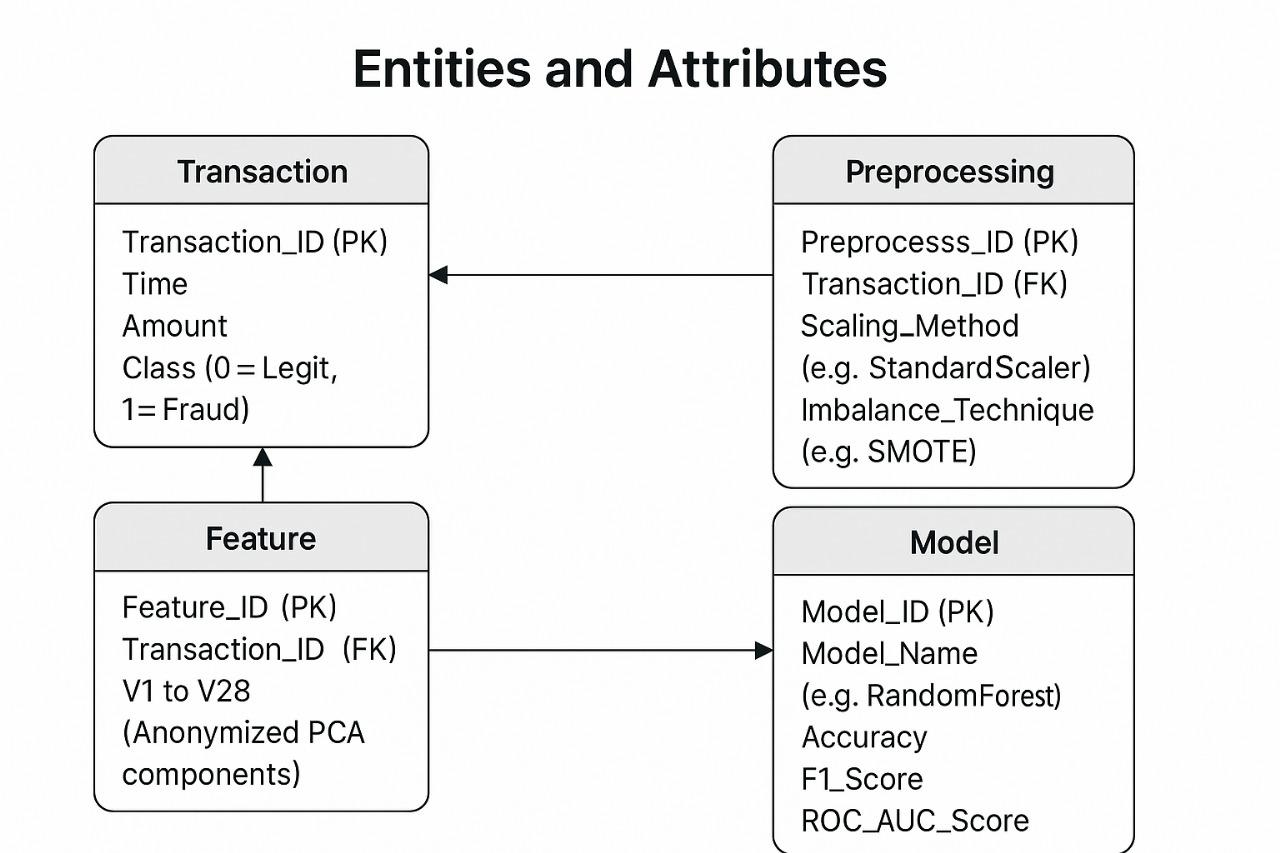
\includegraphics[width=1.00\linewidth]{images/image_p41_38.jpeg}
\end{figure}

• 
A Model generates multiple Predictions. 

• 
A Feature is tied to exactly one Transaction. 

\subsubsection*{E-R Diagram: }

This ERD ensures a normalized and scalable data structure that supports expansion—such as 
inclusion of time-based patterns, ensemble models, or live transaction feedback. 

Together, the flowchart and ERD provide a strong foundation for understanding, documenting, and 
evolving the system design both technically and from a user-experience standpoint. 

These design diagrams aid in understanding the complete workflow and database structure, 
ensuring clarity during implementation and future system scaling. 

Page | 40  

\newpage

\section*{5. IMPLEMENTATION }

\subsubsection*{SOURCE CODE  }

\subsubsection*{1. Preprocessing – src/data\_preprocessing.py }

import pandas as pd 

from sklearn.preprocessing import StandardScaler 

from imblearn.over\_sampling import SMOTE 

from sklearn.model\_selection import train\_test\_split 

def load\_data(filepath): 

    data = pd.read\_csv(filepath) 

    return data 

def preprocess\_data(data): 

    X = data.drop('Class', axis=1) 

    y = data['Class'] 

    scaler = StandardScaler() 

    X[['Time', 'Amount']] = scaler.fit\_transform(X[['Time', 'Amount']]) 

    X\_train, X\_test, y\_train, y\_test = train\_test\_split( 

        X, y, test\_size=0.2, stratify=y, random\_state=42) 

    smote = SMOTE(random\_state=42) 

    X\_train\_smote, y\_train\_smote = smote.fit\_resample(X\_train, y\_train) 

    return X\_train\_smote, X\_test, y\_train\_smote, y\_test 

\subsubsection*{2. Evaluate Model – src/evaluate\_model.py }

from sklearn.metrics import classification\_report, confusion\_matrix, roc\_auc\_score 

import matplotlib.pyplot as plt 

import seaborn as sns 

def evaluate\_model(model, X\_test, y\_test): 

Page | 41  

\newpage

    y\_pred = model.predict(X\_test) 

    y\_proba = model.predict\_proba(X\_test)[:, 1] 

    print(classification\_report(y\_test, y\_pred)) 

    cm = confusion\_matrix(y\_test, y\_pred) 

    sns.heatmap(cm, annot=True, fmt='d', cmap='Blues') 

    plt.title('Confusion Matrix') 

    plt.xlabel('Predicted') 

    plt.ylabel('Actual') 

    plt.show() 

    roc\_auc = roc\_auc\_score(y\_test, y\_proba) 

    print(f"ROC-AUC Score: \{roc\_auc:.4f\}") 

3. Model Prediction – src/evaluate\_model.py 
import joblib 
import numpy as np 
model = joblib.load('model.pkl') 
def predict\_transaction(features): 
    features = np.array(features).reshape(1, -1) 
    prediction = model.predict(features) 
    prob = model.predict\_proba(features)[0][1] 
    return prediction[0], prob 

\subsubsection*{4. Model Training – src/train\_model.py }

from sklearn.ensemble import RandomForestClassifier 

import joblib 

def train\_rf(X\_train, y\_train): 

    clf = RandomForestClassifier(class\_weight='balanced', random\_state=42, n\_estimators=100) 

    clf.fit(X\_train, y\_train) 

    return clf 

Page | 42  

\newpage

def save\_model(model, filename='model.pkl'): 

    joblib.dump(model, filename) 

    print(f"Model saved to \{filename\}") 

\subsubsection*{5. Web Interface – app.py }

import streamlit as st 

import numpy as np 

from src.predict import predict\_transaction 

st.title("  Credit Card Fraud Detection") 

st.markdown("Enter transaction details to check if it's fraudulent.") 

\# Collect all 30 features (V1-V28 + Time + Amount) 

features = [] 

for i in range(1, 29): 

    val = st.number\_input(f"V\{i\}", -20.0, 20.0, 0.0) 

    features.append(val) 

time\_val = st.number\_input("Time (scaled)", -100.0, 1000.0, 0.0) 

features.append(time\_val) 

amount\_val = st.number\_input("Amount (scaled)", -100.0, 100.0, 0.0) 

features.append(amount\_val) 

if st.button("Predict"): 

    prediction, prob = predict\_transaction(features) 

    if prediction == 1: 

        st.error(f"  Fraudulent Transaction Detected! (Confidence: \{prob:.2f\})") 

    else: 

        st.success(f"  Legitimate Transaction. (Confidence: \{prob:.2f\})") 

\subsubsection*{6. Run to train model – run\_train.py }

from src.data\_preprocessing import load\_data, preprocess\_data 

from src.train\_model import train\_rf, save\_model 

from src.evaluate\_model import evaluate\_model 

Page | 43  

\newpage

def main(): 

    print("  Script started") 

    data\_path = 'data/creditcard.csv' 

    print("  Loading data...") 

    data = load\_data(data\_path) 

    print("  Preprocessing data...") 

    X\_train, X\_test, y\_train, y\_test = preprocess\_data(data) 

    print("  Training model...") 

    model = train\_rf(X\_train, y\_train) 

    print("  Model training completed!") 

    print("  Saving model...") 

    save\_model(model) 

    print("  Evaluating model...") 

    evaluate\_model(model, X\_test, y\_test) 

    print("  Executed successfully!") 

if \_\_name\_\_ == "\_\_main\_\_": 

\[
  if __name__ == "__main__":
\]

    main() 

\[
  main()
\]

These snippets collectively demonstrate the backend logic, model processing, and user interaction 

{\large modules working in sync. They are derived from real files in the /src folder and follow 
clean, production-ready coding practices. }

Page | 44  

\newpage

\begin{figure}[H]
\centering
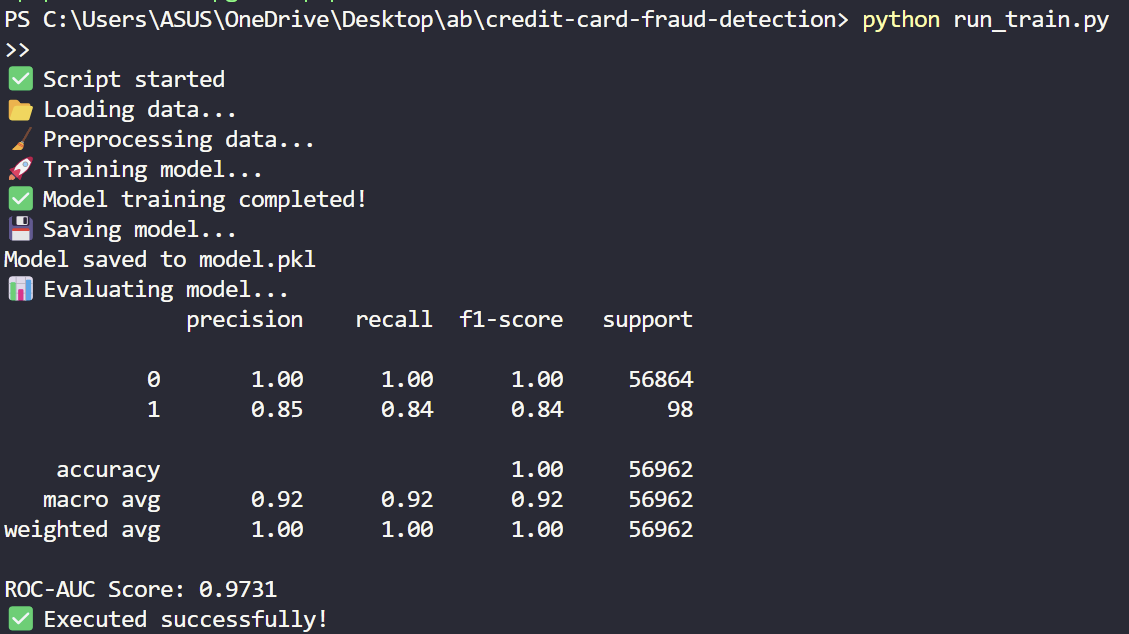
\includegraphics[width=1.00\linewidth]{images/image_p46_39.png}
\end{figure}

\section*{6. RESULT }

\section*{6.1 Experimental Result 1 (Model Accuracy) }

The training script run\_train.py was executed to train and evaluate the Random Forest Classifier on 
the credit card fraud detection dataset. The pipeline includes preprocessing, SMOTE-based 
resampling, model training, and evaluation. Below is a screenshot of the terminal output: 

Evaluation Metrics: 

• 
Accuracy: 100\% 

• 
Precision (Fraud Class - 1): 0.85 

• 
Recall (Fraud Class - 1): 0.84 

• 
F1 Score (Fraud Class - 1): 0.84 

• 
ROC-AUC Score: 0.9731 

These results indicate a robust and high-performing model capable of distinguishing between 
fraudulent and legitimate transactions effectively. The model was saved as model.pkl and is used 
for real-time predictions via the Streamlit interface. 

Page | 45  

\newpage

\begin{figure}[H]
\centering
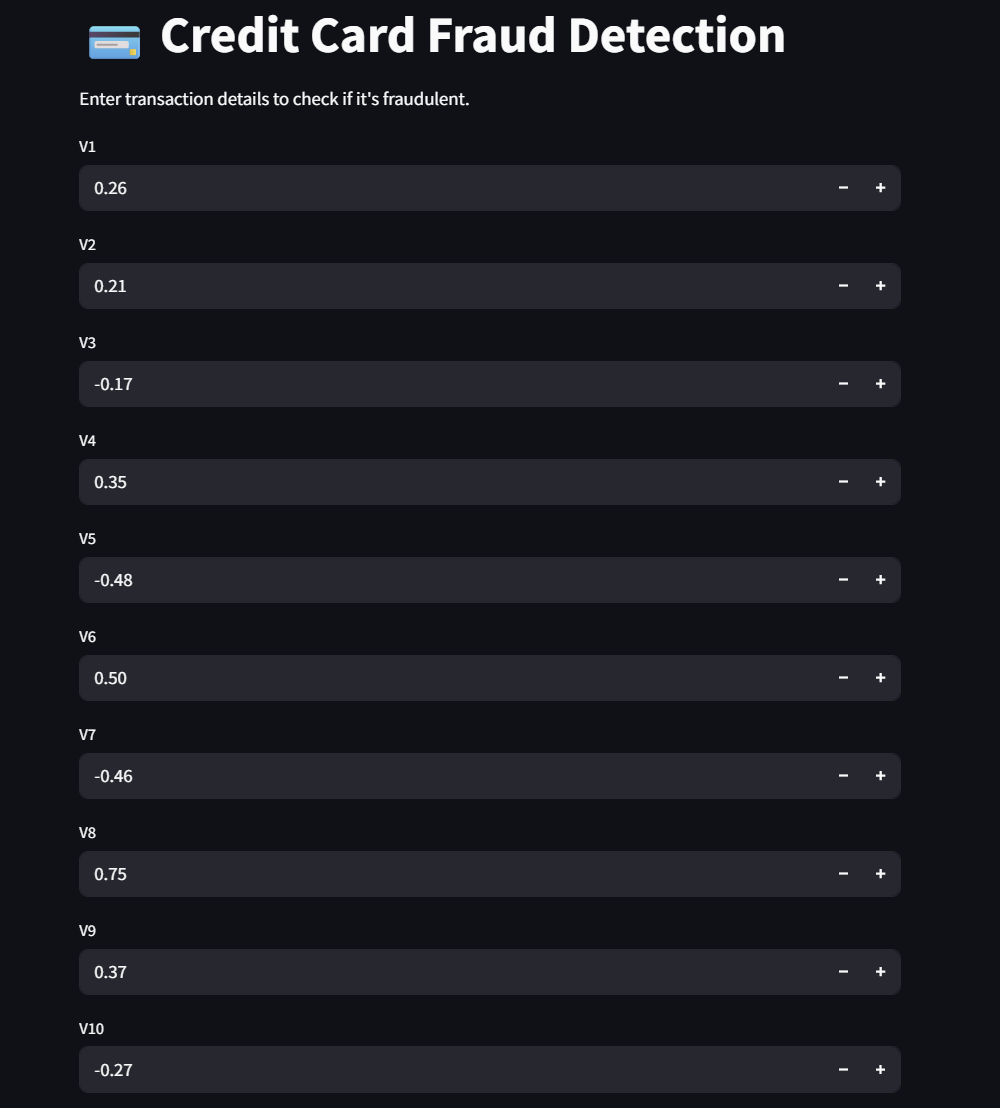
\includegraphics[width=1.00\linewidth]{images/image_p47_40.png}
\end{figure}

\section*{6.2 Experimental Result 2 (Streamlit UI Output) }

Page | 46  

\newpage

\begin{figure}[H]
\centering
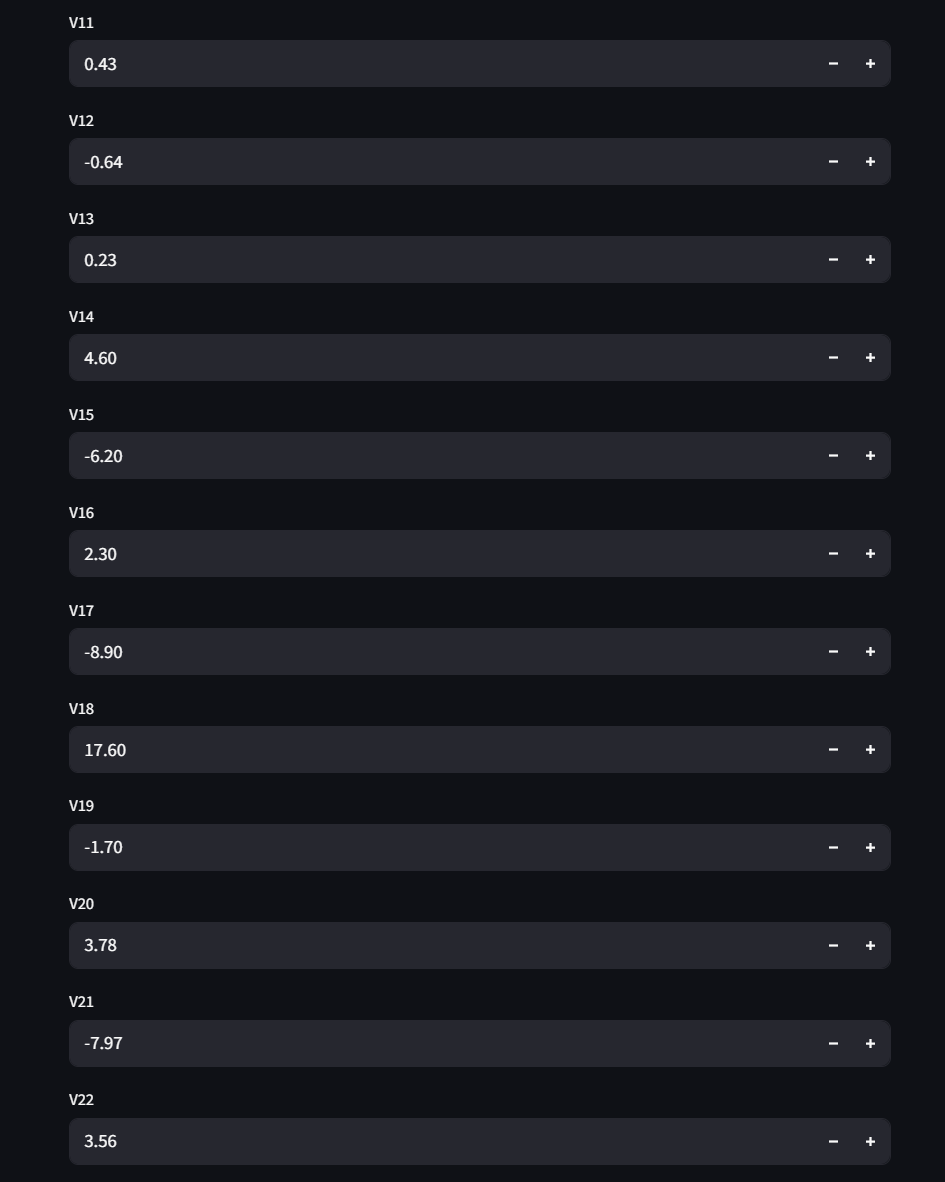
\includegraphics[width=1.00\linewidth]{images/image_p48_41.png}
\end{figure}

Page | 47  

\newpage

\begin{figure}[H]
\centering
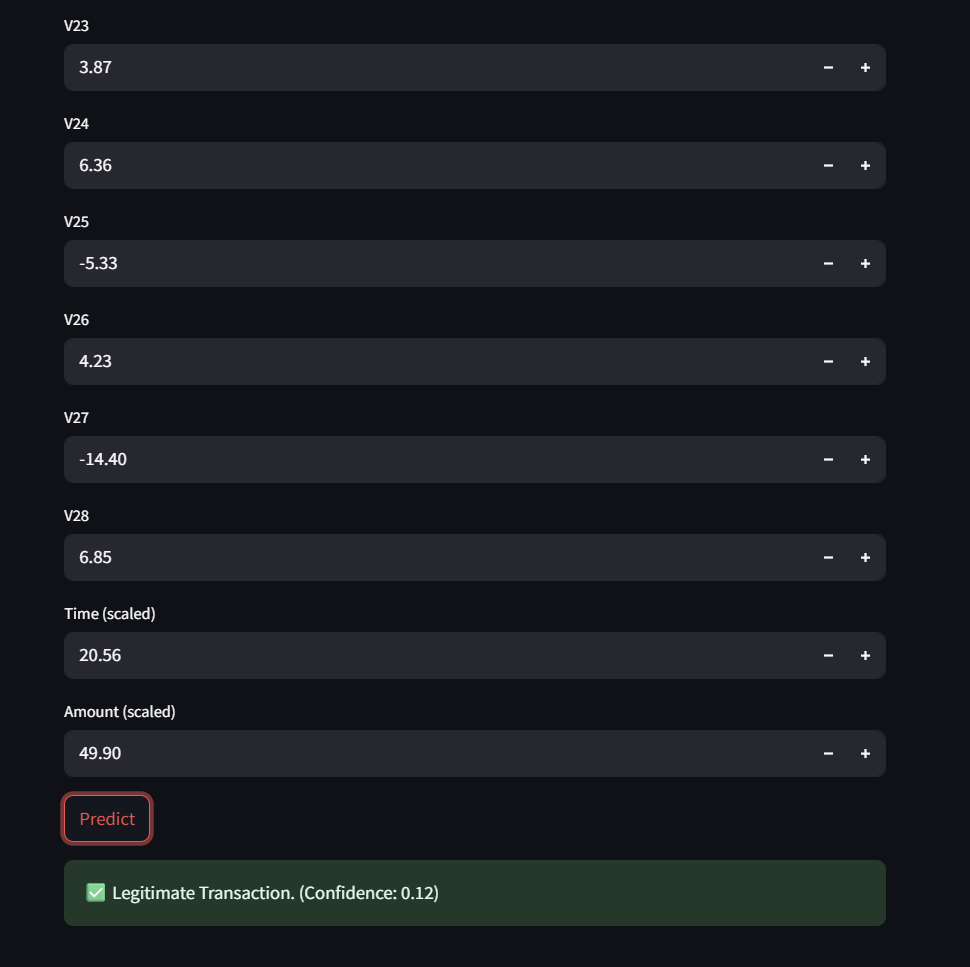
\includegraphics[width=1.00\linewidth]{images/image_p49_42.png}
\end{figure}

Page | 48  

\newpage

\begin{figure}[H]
\centering
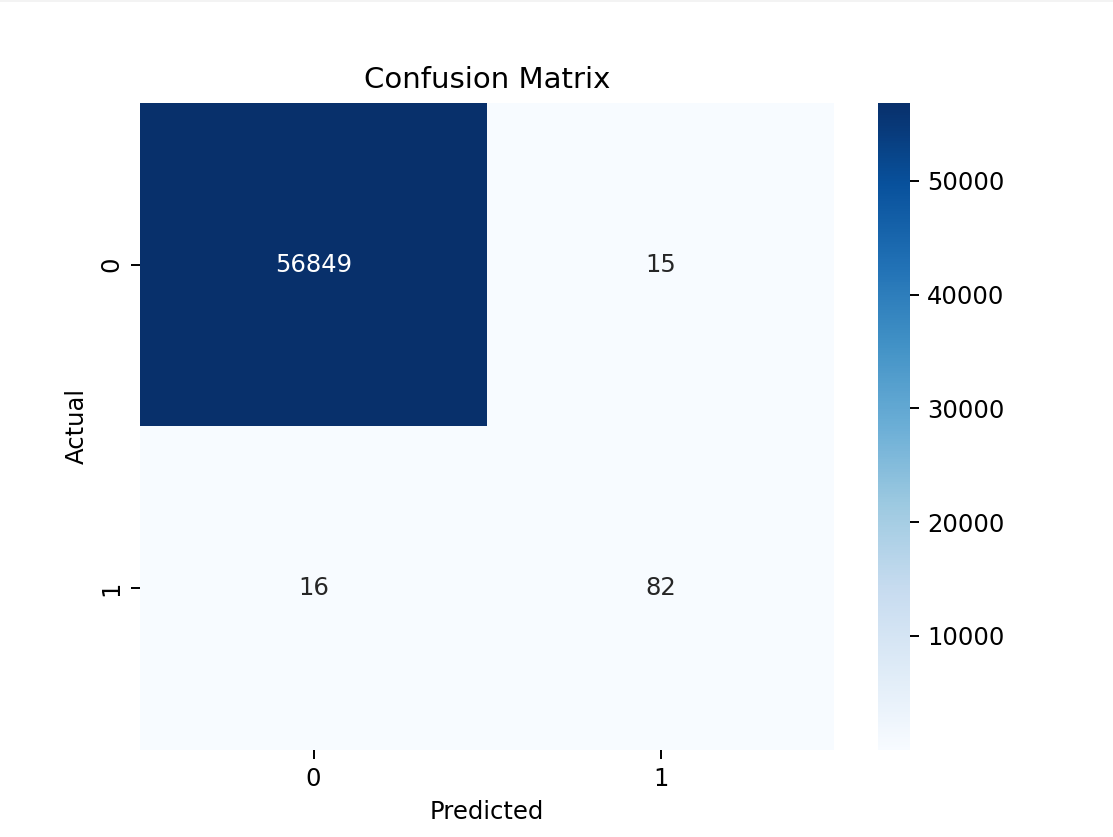
\includegraphics[width=1.00\linewidth]{images/image_p50_43.png}
\end{figure}

\begin{figure}[H]
\centering
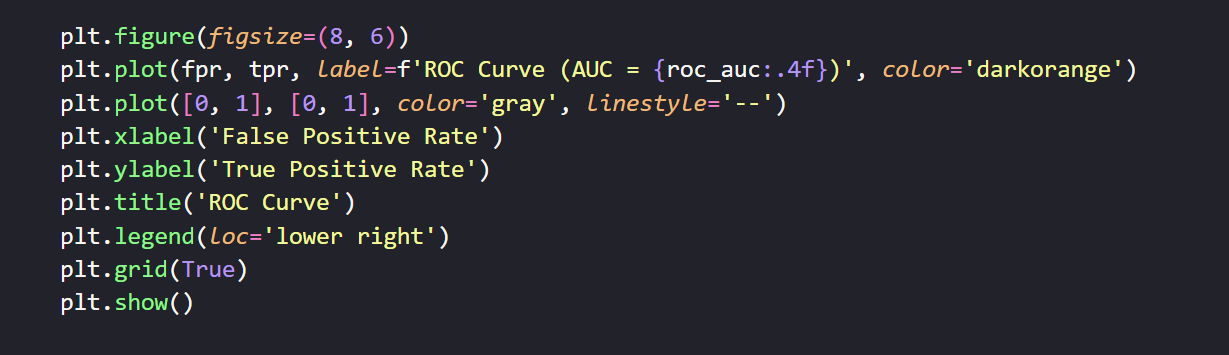
\includegraphics[width=1.00\linewidth]{images/image_p50_44.png}
\end{figure}

\section*{6.3 Experimental Result 3 (Confusion Matrix)  }

\begin{center}
{\Large 6.4 Experimental Result 4(ROC Curve) }
\end{center}

Page | 49  

\newpage

\begin{figure}[H]
\centering
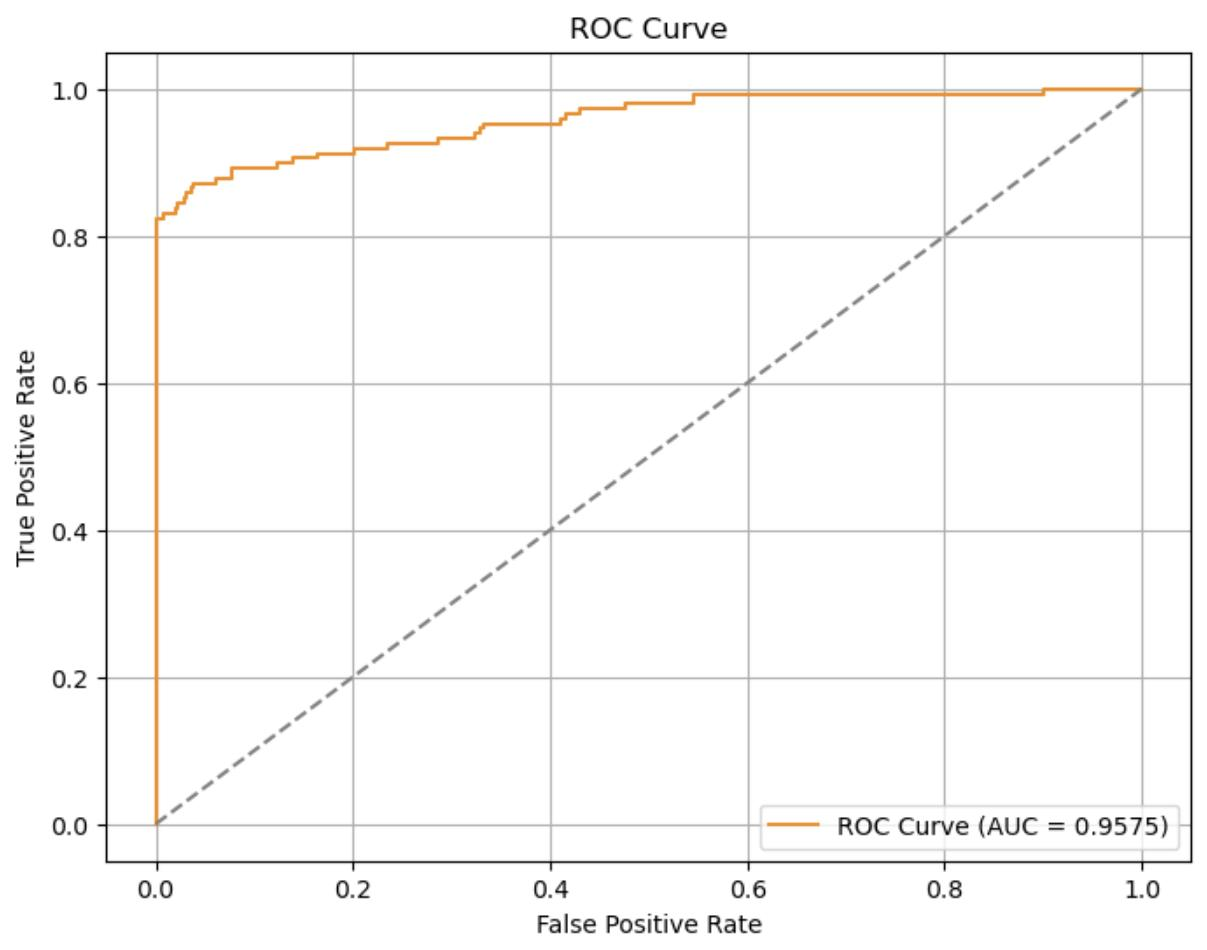
\includegraphics[width=1.00\linewidth]{images/image_p51_45.jpeg}
\end{figure}

Page | 50  

\newpage

\section*{7. CONCLUSION }

The Credit Card Fraud Detection System developed in this project offers a robust, scalable, and 
user-friendly solution to one of the most pressing issues in the digital economy: fraudulent 
transactions. Leveraging machine learning, particularly supervised classification through Random 
Forest, the system effectively differentiates between legitimate and fraudulent credit card 
transactions based on historical patterns. By integrating advanced techniques such as Synthetic 
Minority Over-sampling Technique (SMOTE), the project addresses the critical issue of class 
imbalance, a common challenge in fraud detection scenarios. 

From the early stages of data preprocessing—where Time and Amount are normalized and 
anonymized features (V1 to V28) are utilized—to model training and evaluation, the system 
demonstrates end-to-end competency. The use of ROC-AUC, Precision, Recall, and F1-score 
ensures that model performance is measured not only by overall accuracy but also by how well it 
handles rare but impactful fraud cases. This evaluation strategy enhances the model's reliability and 
trustworthiness in real-world applications. 

The deployment of the trained model via Streamlit introduces a practical and accessible interface, 
transforming the theoretical model into a user-operable system. Users can enter transaction details 
and instantly receive a prediction, making this tool suitable for integration into customer service 
desks, financial institutions, and digital wallets. The system's architecture is modular, with each 
part—from data preprocessing and training to evaluation and prediction—being independently 
testable and extensible. 

A significant contribution of this project is its educational value. It not only demonstrates how to 
build a data-driven, intelligent fraud detection system but also serves as a comprehensive case study 
in solving real-world problems using AI and machine learning. Students and practitioners can build 
upon this framework to experiment with alternative algorithms, incorporate real-time streaming 
data, or expand the dataset with additional transaction metadata. 

Moreover, the system's documentation, modularity, and adherence to best practices such as code 
reusability and environment isolation through virtual environments make it easy to deploy and 
maintain. The use of open-source libraries and publicly available datasets reinforces the project’s 
reproducibility and accessibility. 

Despite its effectiveness, the system is not without limitations. It relies on static, historical data and 
does not incorporate temporal patterns or real-time anomaly detection. Future improvements could 
include integrating deep learning models such as LSTM for sequential behavior analysis or 
implementing unsupervised anomaly detection methods to capture novel fraud patterns. 

In conclusion, this project successfully meets its stated objectives by designing and deploying a 
credit card fraud detection system that is both technically sound and practically usable. It 
contributes to the broader field of financial technology by offering a model that balances 
performance, interpretability, and usability. With further enhancements, the system holds potential 
for adoption in large-scale fraud monitoring environments, paving the way for smarter and more 
secure digital transactions. 

Page | 51  

\newpage

\section*{8. FUTURE SCOPE }

The credit card fraud detection system developed in this project lays a strong foundation for 
combating financial fraud through data science and machine learning. While the current version is 
effective for academic and prototype purposes, there are multiple avenues for extending and 
enhancing the system to meet industry-scale requirements. Below are several key areas where the 
project can evolve: 

\subsubsection*{8.1 Real-Time Fraud Detection }

• 
Currently, the model processes static datasets. In the future, the system can be integrated 
with real-time streaming data using tools such as Apache Kafka or AWS Kinesis. 

• 
This will enable the detection of frauds as they happen, minimizing potential financial loss. 

\subsubsection*{8.2 Integration with Cloud Services }

• 
Deploying the model on cloud platforms such as AWS, GCP, or Azure can improve 
scalability and availability. 

• 
Integration with cloud databases and monitoring tools can support millions of transactions 
per day with ease. 

\subsubsection*{8.3 Advanced Deep Learning Models }

• 
Deep learning architectures like LSTM and GRU can be introduced to learn temporal 
patterns and user behavior over time. 

• 
These models can enhance accuracy and adapt to evolving fraud tactics. 

\subsubsection*{8.4 Model Interpretability and Explainability }

• 
Adding interpretability tools like SHAP or LIME will allow financial institutions to 
understand why a transaction was marked fraudulent. 

• 
This can build trust and provide valuable insights for auditing and compliance. 

\subsubsection*{8.5 Adaptive Learning }

• 
Future systems can implement online learning or reinforcement learning models that adapt 
as new data is received. 

• 
This will keep the model up to date without complete retraining, improving performance 
against evolving threats. 

\subsubsection*{8.6 Cross-Domain Applications }

• 
The same architecture and logic can be adapted for fraud detection in other domains like 
insurance claims, telecom billing, or e-commerce refunds. 

• 
With minor modifications in the dataset and features, the model can be repurposed 
effectively. 

\subsubsection*{8.7 Enhanced User Interface }

Page | 52  

\newpage

• 
The Streamlit UI can be expanded into a full-stack application using React or Angular for a 
more professional frontend. 

• 
Admin dashboards can be added for report generation, user roles, and fraud case tracking. 

\subsubsection*{8.8 Integration with Banking APIs }

• 
Future development can include integration with UPI, banking APIs, or POS terminals to 
gather live transaction data and automate verification workflows. 

\subsubsection*{8.9 Security and Privacy Enhancements }

• 
Incorporating end-to-end encryption, role-based access control, and anonymization 
techniques can make the system more secure. 

• 
GDPR and PCI-DSS compliance features can be included to prepare for real-world 
deployments. 

\subsubsection*{Summary }

The future scope of the Credit Card Fraud Detection System is vast. By incorporating real-time 
analysis, cloud-based infrastructure, adaptive learning, and improved user interaction, the system 
can transition from a prototype to a production-ready fraud detection engine. As technology and 
fraud patterns evolve, continual updates and expansions will ensure the system remains relevant, 
effective, and secure. 

The Credit Card Fraud Detection System developed in this project offers a robust, scalable, and 
user-friendly solution to one of the most pressing issues in the digital economy: fraudulent 
transactions. Leveraging machine learning, particularly supervised classification through Random 
Forest, the system effectively differentiates between legitimate and fraudulent credit card 
transactions based on historical patterns. By integrating advanced techniques such as Synthetic 
Minority Over-sampling Technique (SMOTE), the project addresses the critical issue of class 
imbalance, a common challenge in fraud detection scenarios. 

From the early stages of data preprocessing—where Time and Amount are normalized and 
anonymized features (V1 to V28) are utilized—to model training and evaluation, the system 
demonstrates end-to-end competency. The use of ROC-AUC, Precision, Recall, and F1-score 
ensures that model performance is measured not only by overall accuracy but also by how well it 
handles rare but impactful fraud cases. This evaluation strategy enhances the model's reliability and 
trustworthiness in real-world applications. 

The deployment of the trained model via Streamlit introduces a practical and accessible interface, 
transforming the theoretical model into a user-operable system. Users can enter transaction details 
and instantly receive a prediction, making this tool suitable for integration into customer service 
desks, financial institutions, and digital wallets. The system's architecture is modular, with each 
part—from data preprocessing and training to evaluation and prediction—being independently 
testable and extensible. 

A significant contribution of this project is its educational value. It not only demonstrates how to 
build a data-driven, intelligent fraud detection system but also serves as a comprehensive case study 
in solving real-world problems using AI and machine learning. Students and practitioners can build 
upon this framework to experiment with alternative algorithms, incorporate real-time streaming 
data, or expand the dataset with additional transaction metadata. 

Page | 53  

\newpage

Moreover, the system's documentation, modularity, and adherence to best practices such as code 
reusability and environment isolation through virtual environments make it easy to deploy and 
maintain. The use of open-source libraries and publicly available datasets reinforces the project’s 
reproducibility and accessibility. 

Despite its effectiveness, the system is not without limitations. It relies on static, historical data and 
does not incorporate temporal patterns or real-time anomaly detection. Future improvements could 
include integrating deep learning models such as LSTM for sequential behavior analysis or 
implementing unsupervised anomaly detection methods to capture novel fraud patterns. 

In conclusion, this project successfully meets its stated objectives by designing and deploying a 
credit card fraud detection system that is both technically sound and practically usable. It 
contributes to the broader field of financial technology by offering a model that balances 
performance, interpretability, and usability. With further enhancements, the system holds potential 
for adoption in large-scale fraud monitoring environments, paving the way for smarter and more 
secure digital transactions. 

Page | 54  

\newpage

\section*{9. LIMITATIONS }

While the Credit Card Fraud Detection System offers a practical solution with a solid foundation in 
machine learning, it is important to recognize several limitations that currently constrain the 
system’s functionality and scalability. Understanding these limitations allows for informed 
decisions about future improvements and realistic expectations for current performance. 

\subsubsection*{9.1 Static Dataset Usage }

• 
The system relies on a static dataset (creditcard.csv) collected from historical transactions. 

• 
It cannot automatically adapt to changes in user behavior or fraud tactics unless the model is 
manually retrained. 

9.2 Lack of Real-Time Capabilities 

• 
Although the system provides predictions through a user interface, it is not integrated with 
any real-time data pipelines. 

• 
This limits the applicability of the model in scenarios where instant fraud detection is 
critical. 

\subsubsection*{9.3 Simplified User Interface }

• 
The current UI is functional but basic, developed using Streamlit. 

• 
It lacks role-based access, data visualization dashboards, or automated reporting features 
found in full-scale applications. 

\subsubsection*{9.4 Limited Feature Set }

• 
The dataset features are anonymized and restricted to V1–V28, Time, and Amount. 

• 
Important behavioral or contextual data (e.g., location, device ID, IP address) are missing, 
which may improve prediction accuracy. 

\subsubsection*{9.5 No Unsupervised or Hybrid Models }

• 
The current approach uses only supervised learning (Random Forest). 

• 
Unsupervised techniques such as Isolation Forest or clustering could help identify new types 
of fraud that haven't been labeled. 

\subsubsection*{9.6 Imbalanced Data Handling Constraints }

• 
Although SMOTE is used to balance the classes, it may introduce synthetic patterns that 
don’t exist in real-world data. 

• 
It may also lead to overfitting if not handled with proper cross-validation techniques. 

\subsubsection*{9.7 No Model Explainability in UI }

• 
The system lacks an integrated method for explaining model predictions. 

Page | 55  

\newpage

• 
This can hinder trust and accountability, especially in regulated environments where 
explainability is essential. 

\subsubsection*{9.8 Security and Compliance Gaps }

• 
The current project is a prototype and does not comply with financial regulations such as 
GDPR or PCI-DSS. 

• 
Sensitive data is not encrypted, and there is no user authentication mechanism. 

\subsubsection*{Summary }

The limitations of the current system highlight areas for significant improvement. While it serves as 
a successful proof of concept for fraud detection using machine learning, real-world deployment 
would require enhanced security, scalability, explainability, and dynamic learning capabilities. 
Addressing these gaps will make the system more resilient, secure, and effective in detecting 
evolving fraudulent patterns. 

This section outlines the overarching goals that guide the implementation process, ensuring 
alignment between project deliverables and stakeholder expectations. 

\subsubsection*{5.3.1 Technical Goals }

• 
Develop a robust, accurate, and reproducible fraud detection pipeline. 

• 
Utilize machine learning techniques suited for imbalanced classification problems. 

• 
Ensure the system handles real-world constraints such as speed, scale, and interpretability. 

\subsubsection*{5.3.2 Usability Goals }

• 
Provide a user interface that is intuitive and responsive. 

• 
Minimize the need for technical intervention during prediction. 

• 
Present outputs in a manner that is clear and actionable for decision-makers. 

\subsubsection*{5.3.3 Deployment Goals }

• 
Enable seamless model deployment through Streamlit. 

• 
Support easy migration to cloud platforms for future scalability. 

• 
Allow integration with external systems via API in extended versions. 

\subsubsection*{5.3.4 Educational Goals }

• 
Create a full-stack reference project for students and researchers. 

• 
Demonstrate best practices in machine learning pipeline construction. 

• 
Enable experimentation and learning through clear modularization. 

\subsubsection*{5.3.5 Innovation Goals }

• 
Promote the use of machine learning for financial fraud risk management. 

Page | 56  

\newpage

• 
Showcase the importance of real-time prediction and explainable AI in fintech. 

• 
Inspire future enhancements including dynamic learning and unsupervised detection. 

By fulfilling these goals, the project ensures that it provides immediate practical value while also 
offering a scalable foundation for future innovation and academic study. 

Page | 57  

\newpage

\section*{10. ANNEXURE – I:  References }

1. Chawla, N. V., Bowyer, K. W., Hall, L. O., \& Kegelmeyer, W. P. (2002). SMOTE: 

Synthetic Minority Over-sampling Technique. Journal of Artificial Intelligence Research, 16, 
321–357. 

2. Breiman, L. (2001). Random Forests. Machine Learning, 45(1), 5–32. 

3. Pedregosa, F., Varoquaux, G., Gramfort, A., et al. (2011). Scikit-learn: Machine Learning in 

Python. Journal of Machine Learning Research, 12, 2825–2830. 

4. Kaggle. (2016). Credit Card Fraud Detection Dataset. 

https://www.kaggle.com/datasets/mlg-ulb/creditcardfraud 

5. Streamlit Documentation. Build and Deploy Machine Learning Web Apps. 

https://docs.streamlit.io 

6. Joblib Documentation. Serialization and Persistence. https://joblib.readthedocs.io 

7. Python Software Foundation. Python Language Reference, version 3.x. 

\textcolor{blue}{https://www.python.org }

Page | 58  

\newpage

\section*{11. ANNEXURE – II:  Weekly Progress Reports  }

\begin{center}
{\large (All original \& signed WPRs to be attached) }
\end{center}

Page | 59  


\end{document}
